%------------------------------------------------------------------------------
% Template file for the submission of papers to IUCr journals in LaTeX2e
% using the iucr document class
% Copyright 1999-2013 International Union of Crystallography
% Version 1.6 (28 March 2013)
%------------------------------------------------------------------------------

\documentclass{iucr}
%\documentclass[preprint]{iucr}

\usepackage{epsfig}
\usepackage{graphicx}
\usepackage{amsmath,amssymb}
\usepackage{textcomp}
\usepackage{color,xcolor}
\usepackage{url}
\usepackage[normalem]{ulem}



\newcommand{\todo}[1]{{\color{red}[TODO: "#1'']}}
\newcommand{\inblue}[1]{{\color{black}#1}}
\newcommand{\inred}[1]{{\color{red}#1}}
\newcommand{\ingreen}[1]{{\color{green}#1}}
\newcommand{\replace}[2]{{\color{blue}#1}{\color{blue}\sout{#2}}}





     %-------------------------------------------------------------------------
     % Information about journal to which submitted
     %-------------------------------------------------------------------------
     \journalcode{S}              % Indicate the journal to which submitted
                                  %   A - Acta Crystallographica Section A
                                  %   B - Acta Crystallographica Section B
                                  %   C - Acta Crystallographica Section C
                                  %   D - Acta Crystallographica Section D
                                  %   E - Acta Crystallographica Section E
                                  %   F - Acta Crystallographica Section F
                                  %   J - Journal of Applied Crystallography
                                  %   M - IUCrJ
                                  %   S - Journal of Synchrotron Radiation


\begin{document}                  % DO NOT DELETE THIS LINE

\title{Compensation of heat load deformations using adaptive optics for the ALS upgrade: a wave optics study}

%1) An inclusive (or complete) beamline optimization package to compensate for heat load and other defects with adaptive optics

%2) Adaptive optics to compensate for thermal deformation: theory, simulation and application.

\author[a]{Manuel}{Sanchez del Rio}
\cauthor[a]{Antoine}{Wojdyla}{awojdyla@lbl.gov}{}
\author[a]{Kenneth A.}{Goldberg}
\author[a]{Grant D.}{Cutler}
\author[a]{Daniele}{Cocco}
\author[a]{Howard A.}{Padmore}
\aff[a]{LBNL, 1 Cyclotron Road, Berkeley CA, \country{USA}}

\keyword{Adaptive X-ray Optics}\keyword{Soft X-rays, beamlines}\keyword{wave optics}\keyword{WOFRY}\keyword{OASYS}
 
\maketitle

\begin{synopsis}
A simple and complete one-dimensional wavefront propagation model for beamline analysis is developed in the WOFRY package in OASYS. It is used to analyze how the thermal load of the white beam mirror degrades the wavefront. This can be corrected by a adaptive mirror, with some limitations that are studied.
\end{synopsis}

\begin{abstract}
We have developed a realistic wave optics simulation method to study how wavefront distortions originated by heat load deformations can be corrected using adaptive X-ray optics. Several planned soft X-ray and tender X-ray insertion-device beamlines in the Advanced Light Source upgrade rely on a common design principle. A flat, first mirror intercepts the white beam; vertical focusing is provided by a variable-line-space monochromator; and horizontal focusing comes from a single, pre-figured, adaptive mirror. 
A variety of scenarios to cope with thermal distortion in the first mirror are studied by finite-element analysis. We analyze the degradation of the intensity distribution at the focal plane and model the adaptive optics that correct it. We report the range of correctable wavefront errors across the operating range of the beamlines in terms of mirror curvature and spatial frequencies. The software developed is a one-dimensional wavefront propagation package made available in the OASYS suite, an adaptable, customizable and efficient beamline modeling platform.
\end{abstract}

%
%
%
\section{Introduction}
\label{sec:intro}  

Quantitative calculation and evaluation of the parameters related to X-ray optics are of great importance for designing, building and exploiting new beamlines. These calculations allow testing of the design parameters in a virtual computer environment where advantages and limitations can be simulated accurately. The optics imperfections play a fundamental role in the simulations and often constitute the limiting factor of beamline performance. Deformations of the optical elements due to heat load need to be controlled and in some cases corrected, therefore optics simulations and engineering modeling of the thermal deformations by finite element analysis (FEA) have to be developed in parallel. 

Simulations of the beamline optics can be done in different degrees of approximation and effort, starting from analytical formulas, performing ray-tracing, and also wavefront propagation \cite{hyerarchical}. Different packages for such simulations are available in the OASYS suite \cite{codeOASYS}. For beams of incoherent photons, the ray-tracing technique is suitable for most purposes. If the X-ray beam is highly coherent, like in soft X-ray beamlines of the upgraded ALS facility discussed in this paper, a pure wave-optics simulation is sufficient. For hard X-rays, where the coherent fraction for upgraded facilities is usually a few percent, simulations require using hybrid methods \cite{hybrid} or more sophisticated partial coherence algorithms such as Monte Carlo sampling \cite{Chubar2011b} and Coherent Mode Decomposition \cite{glassEPL}. 

A common design being implemented in several insertion-device beamlines at the upgraded Advanced Light Source (ALS-U) consists of a horizontally deflecting, cooled, planar, M1 mirror to absorb a large part of the white beam power and deflect the light out of the bremsstrahlung cone. This is followed by a horizontally focusing adaptive mirror M3, that focuses and corrects wavefront errors. A variable-line-space (VLS) grating monochromator is placed in between to disperse and focus the beam in the vertical plane \cite{reininger2005}. The monochromator is decoupled from the M1-M3 system. 

In this paper we study the ability of the adaptive mirror M3 to compensate wavefront aberrations caused by power-load-induced thermal distortions on M1. The white beam impinges on M1 after being shaped by high power slits, but the power absorbed by the mirror system may produce significant mirror surface deformation that degrades the beam quality. 
A variety of thermal distortion scenarios were implemented from finite-element analysis models using realistic undulator power spectra and cooling strategies under consideration by the project.
In the case of interest of ALS-U, the coherent fraction is high enough (about 0.8 for the case under study, a 4 m undulator at 230.888 eV) to justify a calculation with a fully coherent beam. Moreover, in this case, as is common with synchrotron beamlines, the optics in the horizontal and vertical planes are decoupled, thus, separated modeling of the horizontal and vertical planes is justified. The 1D modeling is orders of magnitude less demanding in computational resources than 2D calculations, therefore it is always recommended to start a wave optics simulation in its simpler 1D form. We present here the fundamentals of a 1D wave propagation model implemented in the WOFRY \cite{codeWOFRY} tool in OASYS.

The 1D waveoptics propagation model is also well adapted to study optimization problems, because a parametric study (scan of a single variable) or multiple optimizations require running many single simulations. In our case, the M3 correction profile is optimized and expressed as a function of the input signal required by the actuators that shape the optics. 
Using data from a 18-channel adaptive X-ray mirror prototype, we implemented mirror shape-control algorithms designed to restore the focused beam and optimize the Strehl ratio.

The paper is organised as follows. In section~\ref{sec:wofry} we describe in detail the methods and algorithms implemented in the WOFRY 1D simulations concerning the sources, wave propagators for free space, and optical elements. In section~\ref{sec:main} we describe the system under study, that corresponds to the parameters of the FLEXON beamline being developed for ALS-U. We further discuss finite-element modeling of the M1 surface thermal deformation originating from the absorbed power. We show (section~\ref{sec:scans}) how the adaptive X-ray optics (AXO) can compensate the errors using an ad-hoc computed mirror profile compatible with the AXO control system. In section~\ref{sec:2D} the complete beamline is simulated using a 1D wavefront propagation model by combining the results of the horizontal and vertical planes. A final summary is in section~\ref{sec:summary}.

%
%
%
\section{Simplified 1D wavefront modeling for synchrotron beamlines}
\label{sec:wofry}

A wavefront simulation consists of the creation of a wavefront with some characteristics (geometry, wavelength), its propagation in free space and its modification by the optical elements (slits, mirrors, etc). We restrict the description here to a 1D model in the ($x,y$) plane, with $y$ as the propagation direction (optical axis) and $x$ as the direction transverse to the beam propagation to analyze (usually the of horizontal or vertical plane). The wavefront is represented by the electric field of a monochromatic component (angular frequency $\omega$, wavelength $\lambda$, wavenumber $k = 2 \pi / \lambda$ or photon energy $W$) at a position $y=0$ along the propagation direction. This electric field or electric disturbance is a complex scalar $E(x;y=0,\omega)$ or, in case of polarized beams, two complex scalars, one for $\sigma$ and the other for $\pi$ polarization. The wavefront intensity is the square of the modulus of the amplitude: $I=|A \exp{(i\phi)}|^2=A^2$. 

\subsection{Modeling sources}
\label{sec:sources}

\subsubsection{Simple waves: plane, spherical and Gaussian}

The simplest wavefront is a plane wave, with constant complex amplitude for any $x$ coordinate: 
\begin{equation}
   E(x;y=0,\omega)=E_0=A_0 e^{i \phi_0},
\end{equation}
where $E_0$ is a complex value that can be expressed in its constant real amplitude $A_0$ and a constant phase $\phi_0$. A plane wave is infinite along the $x$ direction. However, when representing a wavefront spatially, in simulation, the electric field has to be sampled over an array of discrete values of complex amplitude, and they are necessarily defined over a finite $x$ interval. 

A spherical wave (strictly speaking a circular wave in 1D, but we keep the terminology used in 2D) emanates from a fixed point and has a constant complex amplitude over a sphere of a given radius $R$. Obviously it cannot be represented at the source point ($y=0$, center of the sphere) and our wavefront must be sampled at a given distance $y=R$ and over a line perpendicular to the radius and tangent to the sphere. At $x=0$ (a point in the sphere) the field has a constant value equal to the value at the surface. But at a $x{\ne}0$, over a range of $x$-values $x{\ll}R$ (i.e. for small numerical apertures, NA) the distance from $x$ to the sphere parallel to the $y$ direction gives an optical path that modifies the phase by $k ~\Delta x$. It is easy to deduce that the wavefront in the line tangent to the sphere has the expression
\begin{equation}
\label{eq:sphericalWave}
    E(x;y=R,\omega)  = E_0 e^{i k x^2 / (2 R)}.
\end{equation}

% possible figure: 
% https://slideplayer.com/slide/730247/2/images/10/Spherical+wave+propagation.jpg

A Gaussian beam at the source position $y$=0 has constant phase and intensity following a Gaussian distribution with standard deviation $\sigma_I$, thus the electric disturbance is: 
\begin{equation}
\label{eq:gaussianSource}
    E(x;y=0,\omega) = E_0 e^{-x^2 / (4 \sigma_I^2)}
\end{equation}


\subsubsection{A simplified model for the undulator source}
\label{sec:undulator}

A single electron (or filament beam) traveling in an undulator with pure sinusoidal magnetic field in one direction will produce a complicated wavefront with geometry that varies as a function of the photon frequency (see, e.g., Ref.~\cite{elleaume}). At the resonance energy the angular emission in the far field can be approximated by a Gaussian function of width \cite{elleaume}
\begin{equation}
\label{eq:undulatorDivergence}
    \sigma'_u \approx\sqrt{\frac{\lambda}{2 L}},
\end{equation}
with wavelength of the photons at the undulator resonance, $\lambda$, and undulator length, $L$. At the source point, the size of the source can also be approximated by a Gaussian of width
\begin{equation}
\label{eq:undulatorSize}
    \sigma_u \approx\sqrt{\frac{\lambda L}{2 \pi^2}} = \frac{\lambda}{2 \pi} \frac{1}{\sigma'}.
\end{equation}

A  simplification of the undulator radiation in the far field consists in a spherical wave (Eq.\ref{eq:sphericalWave}) with origin in the undulator center modulated with an amplitude that follows the Gaussian in Eq.~\ref{eq:undulatorDivergence}, therefore
\begin{equation}
    \label{eq:undulatorBySphericalWave}
    E(x;y=y_0,\lambda) = E_0 e^{i k x^2 / (2 y_0)} e^{-x^2/(4 \sigma'_u{}^2 y_0^2)}.
\end{equation}

A second way to simulate the undulator is considering a Gaussian source as defined in Eq.~\ref{eq:gaussianSource} with $\sigma_I=\sigma_u$. Note that propagating this approximation of the undulator as a Gaussian source to a screen at $y=y_0$ does not reproduce the result in Eq.~\ref{eq:undulatorBySphericalWave} because Gaussian propagation implies a product of sigmas (emittance) of $\lambda / (4 \pi)$ whereas for undulator radiation the emittance is approximately $\lambda / (2 \pi)$ (Eq.~\ref{eq:undulatorSize}). For practical purposes, the Gaussian source approximation can be used for optical systems accepting a high NA, whereas for systems of small NA, as used in this paper, the spherical wave approximations may be preferred.


\subsection{Modeling propagation in free space}
\label{sec:propagation}

For simulating the beamline, the wavefront at the source has to be created using the methods in section  \ref{sec:sources}, and then the optical elements modify sequentially the wavefront using the algorithms described in section \ref{sec:elements}.  But the wavefront evolves when transported in free space from element to element. We use here two propagators. 

\subsubsection{Direct implementation of integral Rayleigh-Sommerfeld propagator}
\label{sec:integralPropagator}

The Rayleigh-Sommerfeld propagator for small-angle approximation expresses the electric field at a spatial point $\vec{r}'$ as an integral of the electric field at a spatial point $\vec{r}$ \cite{goodmanfourier}
\begin{equation}\label{eq:RSpropagator}
E(\vec{r}') =  \frac{k}{2 \pi i} \int \frac{E(\vec{r})}{|\vec{r}'-\vec{r}|} e^{ i k |\vec{r}' - \vec{r}|  }  d\Sigma,
\end{equation}
where the integral is made over the domain of the source (the surface $\Sigma$). 
This propagator can be applied to numerical discrete 1D wavefronts, and the integral reduces to a sum
\begin{equation}\label{eq:discreteRSpropagator}
E(x_1,y_1) \approx \frac{k}{2 \pi i \Delta y}  \sum_{i=0}^{N-1}  E(x_{0,i},y_{0,i}) e^{i k \sqrt{(x_1 - x_{0,i})^2 + (y_1 - y_{0,i})^2} }  \Delta x_0,
\end{equation}
where $\Delta y$ is the mean value of the denominator in the integral in Eq.~\ref{eq:RSpropagator}.
Note that one sum over the $N$ points of the sampled incident wavefront has to be done for each coordinate at the transported wavefront, thus the number of operations is of the order $N^2$. This simple propagator gives flexibility to define different gridding and limits permitting the adjustment of the spatial domain or window and spatial resolution when working with converging or divergent wavefronts. Moreover, the propagated wavefront can be computed in a plane (or line) non parallel to the incident one, a feature that is exploited in sections~\ref{sec:grazingReflector} and \ref{sec:grating}. 


\subsubsection{Fresnel propagator using FFT: The zoom propagator}
\label{sec:zoomPropagator}


The Fresnel propagator is obtained by making a Taylor expansion of the quadratic phase in Eq.~\ref{eq:RSpropagator}: 
\begin{equation}\label{eq:fresnelPropagator}
E(x;y_1) =  \frac{e^{i k (y_1-y_0)}}{\sqrt{i \lambda (y_1-y_0)}} \int E(x';y_0) e^{ \frac{i k}{2 (y_1-y_0)}  (x-x')^2  }  dx'.
\end{equation}

The Fresnel integral propagator can be seen as convolution of the wavefield with a Gaussian kernel. One can write Eq. \ref{eq:fresnelPropagator} in convolution form, involving \inblue{a Fourier transform $\mathcal{F}$ and an inverse Fourier transform $\mathcal{F}^{-1}$}\cite{goodmanfourier}:
\begin{equation}\label{eq:fft}
E(x; y_1) = \inblue{P^G} \mathcal{F}^{-1}\Big\{ \mathcal{F}\{E\} K \Big\},
\end{equation} 
where \inblue{$E$ is the electric perturbance at $y_0$ $E(x;y_0)$, $P^G=e^{i k (y_1-y_0)}$ is a global phase and $K=e^{-i \pi \lambda (y_1-y_0) u^2}$ is the Gaussian Kernel } that comes from the inverse Fourier Transform of the exponential inside the integral in Eq.~\ref{eq:fresnelPropagator}, being $u$, the conjugated variable of $x$.
The real benefit of using this scheme comes from the use of Fast Fourier Transforms, that reduce the number of operations from $N^2$ to $N \log_2 N$. Its use is essential when doing simulations in 2D, because the direct calculation of the integral lead to $N^4$ operations at the limit of calculation power of usual laptop computers. However, the FFT implementation requires that the gridding and spatial domain of the incident and transported wavefronts must be equal. This is a problem when a wavefront is propagated to a focal point: the gridding of the incident wavefront used at the image provides a poor resolution because most of the intensity is concentrated in a very few pixels. A clever solution to this problem is presented by J.D. Schmidt \cite{schmidt} that makes possible to calculate the propagated field in a ``zoomed'' window, thus permitting optimizing the wavefront sampling in cases for propagating highly convergent or divergent wavefronts. The problem reduces to a convolution problem of the unpropagated field field $E(x;y_0)$ affected by a phase $P$ with a kernel $K$, and the result affected by a global phase $P^G$: 
\begin{equation}
E(x; y_1) = P^G \mathcal{F}^{-1} \Big\{ \mathcal{F} \big\{ E~~P \big\} K \Big\},
\end{equation}
where
\begin{equation}
P^G =  \frac { e^{ik(y_1-y_0) }}{\sqrt{m_x} }e^{i \frac{k}{2 (y_1-y_0)} \frac{m_x - 1}{m_x}x_2^2},
\end{equation}
\begin{equation}
P = e^{i \frac{k}{2(y_1-y_0)} (1-m_x)x_1^2 },
\end{equation}
\begin{equation}
K = e^{-i \pi \lambda (y_1-y_0) \frac{u^2}{m_x} }.
\end{equation}
The term $m_x$ is the magnification (zoom) factor. 
Note that setting unity magnification $m_x=1$, one obtains the standard Fresnel propagator (Eq.~\ref{eq:fft}).

\subsection{Modeling optical elements}
\label{sec:elements}

In cases where the distance between elements is significantly greater than the mirror sizes, the optical elements can be approximated as thin elements (zero thickness along the $y$ axis), and their effect can be encapsulated in a complex transmission amplitude,
\begin{equation}
    \label{eq:thinelement}
    R(x;\omega)=r(x;\omega) e^{i \rho(x,\omega)}.
\end{equation}
Therefore, the wavefield after an optical element placed at position $y=y_0$ will be the wavefield at $y_0$, just before the interaction, multiplied by the complex transmission:
\begin{equation}
    E'(x;y=y_0,\omega) = E(x;y=y_0,\omega) R(x;\omega)
\end{equation}


\subsubsection{Apertures (slits, beamstops and element dimension)}
\label{sec:aperture}

A generic aperture is a mask that transmits a part of the wavefront in a range $[x_{min},x_{max}]$ and absorbs the rest. It can be
\begin{equation}
R(x;\omega) =
\left\{
\begin{matrix}
A,  & \mbox{~~if~~} x_{min} \le x \le x_{max}
\\ 
1 - A, & \mbox{~~elsewhere}
\end{matrix}
\right.
\end{equation}
When the element is a slit, then $A=1$. If it is a beamstop, then $A=0$. If we deal with an optical element of finite length $L$ placed at a grazing incidence angle $\theta$, it acts as a slit of aperture equal the projection of the length on the $x$ axis: $A=1$, $x_{min}=-(L/2) \sin \theta$ and $x_{max}=(L/2) \sin \theta$. 

\subsubsection{Ideal lens}
\label{sec:idealLens}

We can define an ideal lens as a focusing device that converts a plane wave into a spherical wave collapsing to the focus at a distance $f$ from the ideal lens position. Therefore
\begin{equation}
    R(x;\omega) = e^{-i k~x^2/(2 f)}
\end{equation}

\subsubsection{Ideal reflector}
\label{sec:idealReflector}

Let us consider a perfectly reflecting surface (no absorption) with a profile $h(w)$ with $h$ the elevation (height) and $w$ the linear coordinate in a reference frame attached to the reflector with origin in the reflector's center. A plane reflector has $h(w)=0$ and, for example, a circular mirror of radius $R$ has $h(w)=R-\sqrt{R^2 - w^2}$. The profile $h(w)$ can also match a deformation originated for instance by heat load or a mirror surface error (waviness).

If the reflector is set with an incident angle $\theta$, with the propagation axis $y$, the change of optical path is $\Delta y = 2 h(w) \sin \theta$, $w=x/\sin\theta$, with a consequent phase shift $\Delta \Phi = - k \Delta y $, therefore for the ideal reflector
\begin{equation}
\label{eq:idealReflector}
    R(x;\omega) = e^{-2 i k h(w) \sin \theta}.
\end{equation} 

This model of ideal reflector as a thin object  can be used for any reflecting shape (circular, ellipse, etc.) but the intrinsic aberrations are not correctly considered.  The main reason is the incidence angle $\theta$ is not constant along the mirror profile thus Eq.~\ref{eq:idealReflector} is not exact. A model for a ``grazing reflector" that solves this problem is presented in the next section \ref{sec:grazingReflector}.

A reflector of a finite size can be decomposed in two elements: the ideal reflector described here, followed (or preceded) by the aperture as described in \ref{sec:aperture}.

\subsubsection{Grazing reflector}
\label{sec:grazingReflector}

The method used for the {\it ideal reflector} does not account for mirror aberrations and it is not exact when dealing with mirror errors because the optical path is approximated. These effects are more important for elements in grazing incidence, where the {\it thin object} approximation is not valid. A solution for that consists in using the propagator in Sec.~\ref{sec:integralPropagator} to propagate the incident wavefront until the points in the mirror surface $(w,h)$. Let be $p$ the distance from the wavefront $E_0(x,;y=0,\omega)$ to the center of the mirror placed at a grazing incidence $\theta$ with the optical axis. In the mirror reference frame, the wavefront coordinates are $(w_s, h_s) =(-p \cos \theta, p \sin \theta) + (x \sin \theta, x \cos \theta)$. It is straightforward to extend the integral propagator (Eq.~\ref{eq:discreteRSpropagator}) to calculate the propagated field at the surface points $(w,h)$ by summing over all points of the input wavefront. Once the electric perturbation at the mirror surface is known, another propagation is performed using the same principle, to the image plane placed at a distance $q$ from the mirror center.

\subsubsection{Gratings}
\label{sec:grating}

A grating produces a diffraction of the incident beam that is dependent on its wavelength. It is expressed by the grating equation:
\begin{equation}
    m \lambda g = \sin\alpha + \sin\beta,
\end{equation}
with $\alpha$ the incidence angle (measured with respect to the normal), $\beta$ the reflection angle, with opposite sign of $\alpha$ if it lies at the other side of the normal, $m$ the diffraction order (positive for inside reflection, i.e., $\alpha \ge |\beta|$),
%(note than in SHADOW is the contrary, inside orders are negative)
$\lambda$ is the photon wavelength, and $g$ is the grating groove density, which is a function of $w$ for VLS gratings: $g = g_0 + g_1 w + g_2 w^2 + ...$ with $g_0 = 1/d_0$ the lines per unit of length at the grating center ($d_0$ the distance between two grating lines).

The simulation of a grating using a thin object model (Eq.~\ref{eq:idealReflector}) is difficult because in addition to the geometric optical path it is necessary to account for the wavelength-dependent component. We use here an approach that is exact, except for accounting for the diffraction efficiency, which consisting of sampling the grating as a numeric mesh and apply the ``grazing reflector." 
This model also permits to study line spacing errors together with height errors of the substrate. It is important not to undersample the grating (e.g., we must include several points per period) and orientate the incident and image wavefronts with the correct angles $\alpha$ and $\beta$.

%
%
%
\section{Simulation of ALS-U generic undulator beamline}
\label{sec:main}

Four new undulator beamlines are being designed for the ALS-U project. The different scientific cases imply particular selection of the insertion devices and beamline optics. However, most of the beamlines (or beamline branches) follow a similar scheme: 1) undulator source; 2) white beam, flat mirror M1, deflecting horizontally; 2) plane mirror M2, vertically deflecting to work in tandem with the grating; 3) a VLS (varied line spacing) grating on a flat substrate that vertically disperses the beam and focuses the first diffracted order to the exit-slit plane; and 4) a horizontally-deflecting, plane-elliptical mirror M3 that focuses the source to exit slit plane. The mirror M3 is an adaptive x-ray optic (AXO) equipped with a piezoelectric bimorph system that enables corrections of the $x$-direction wavefront deformations introduced upstream of it.

The goal of this paper is to study the ability of the AXO mirror to correct the distortions produced by thermally-induced deformation of M1.


\subsection{Power loaded by the white mirror M1}

The total power $P$ emitted by an undulator is (e.g., \cite{elleaume})
\begin{equation}
    P[\textrm{W}] = 72.5688 (E_e [\textrm{GeV}])^2  I[\textrm{A}]  N_u  K^2 / \Lambda[\textrm{mm}],
\end{equation}
where $K$ is the undulator deflection parameter, $N_u$ the number of periods, $\Lambda$ the undulator period, $I$ is the storage ring current, and $E_e$ is the storage ring energy. From this equation we can deduce that the maximum of power is obtained at maximum of $K$ corresponding to the minimum of the energy for a given harmonic.  We have selected the case of the FLEXON beamline because the proposed insertion device will deliver high power and the beamline optical design follows the structure described above. Therefore, it constitutes the worst case that requires the most demanding actions to minimize the deformations (in M1) and correct the distortions (in M3). The FLEXON beamline will incorporate a Delta undulator \cite{deltaundulator} with $\Lambda$=~28.8~mm, $N_u$~=~137 and $K_{max}$~=~3.07, emitting a total power of $P$~=~6507~W in the ALS-U storage ring (2~GeV, 0.5~A).

The white beam mirror M1 is placed at a distance 13.73~m from the source, has a grazing angle of 1.25\textdegree, and is gold coated. The distribution of the heat load on the mirror depends on undulator parameters (deflection parameters, horizontal $K_h$, vertical $K_v$, and phase $\Phi$). Depending on the desired polarization, these parameters take different values. For example, for horizontal linear polarization, $K_h=0$; vertical linear polarization, $K_v=0$; linear polarizartion at 45\textdegree $K_h=K_v$, $\Phi=0$; circular polarization $K_h=K_v$, $\Phi=90$\textdegree. In Fig.~\ref{fig:M1powerdensity}, the incident power density on the M1 mirror surface is plotted for $K=\sqrt{K_h^2 + K_v^2}=3.07$ in various polarization states. The undulator tuned at K=3.07 will have its first harmonic at photon energy 230.888 eV which central cone divergence is 32~$\mu$rad rms.

\begin{figure} 
\label{fig:M1powerdensity}
%\begin{center}
%\begin{tabular}{l} 
%   a)~~~~~~~~~~~~~~~~~~~~~~~~~~~~~~~~~~~~~~~~~~~~
%   b)~~~~~~~~~~~~~~~~~~~~~~~~~~~~~~~~~~~~~~~~~~~~\\
%   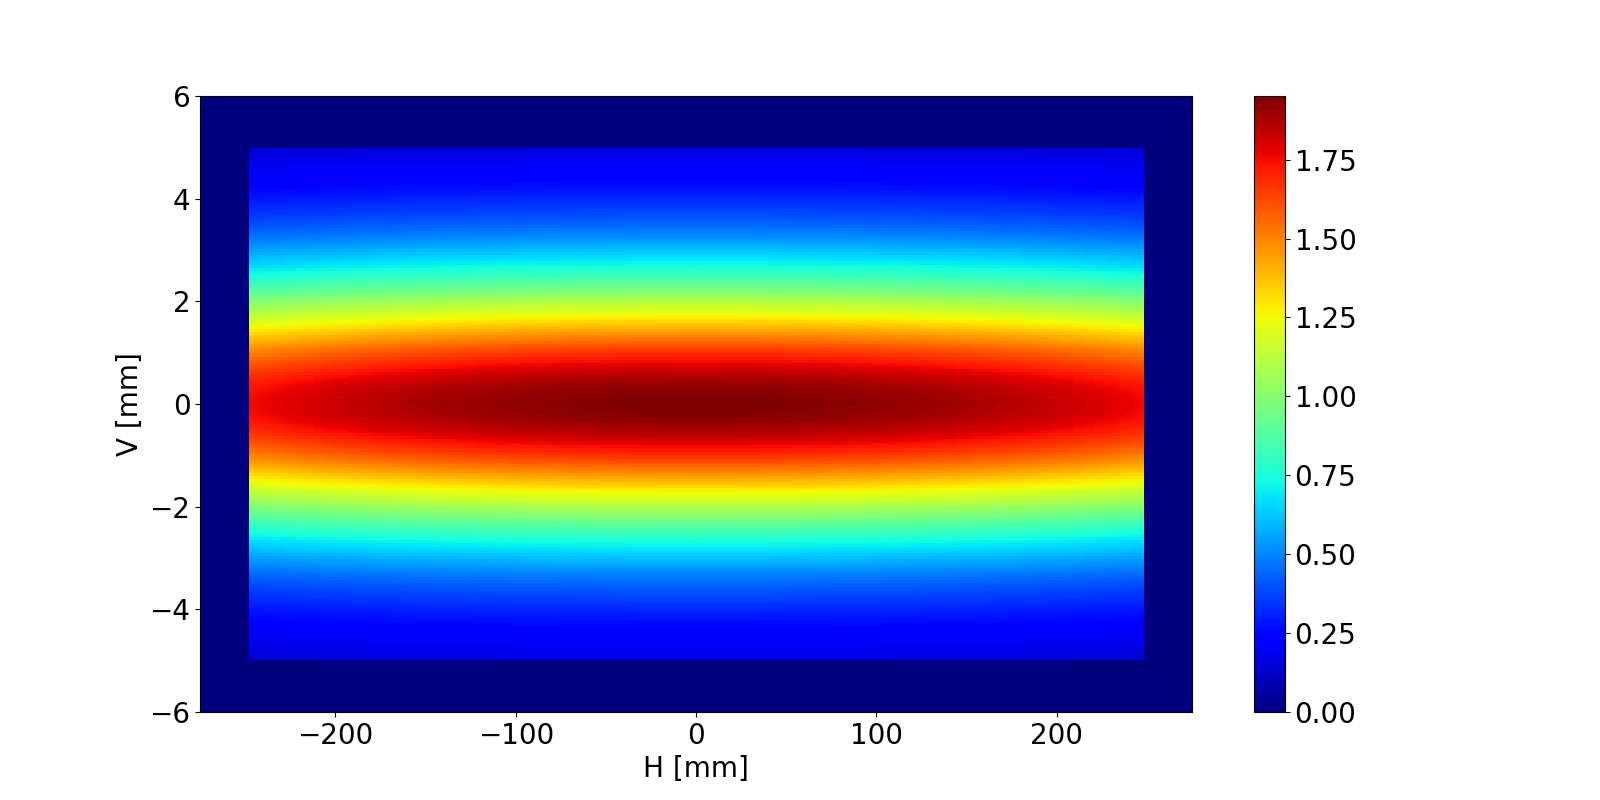
\includegraphics[width=0.45\textwidth]{figures/powerdensityKv.png}
%   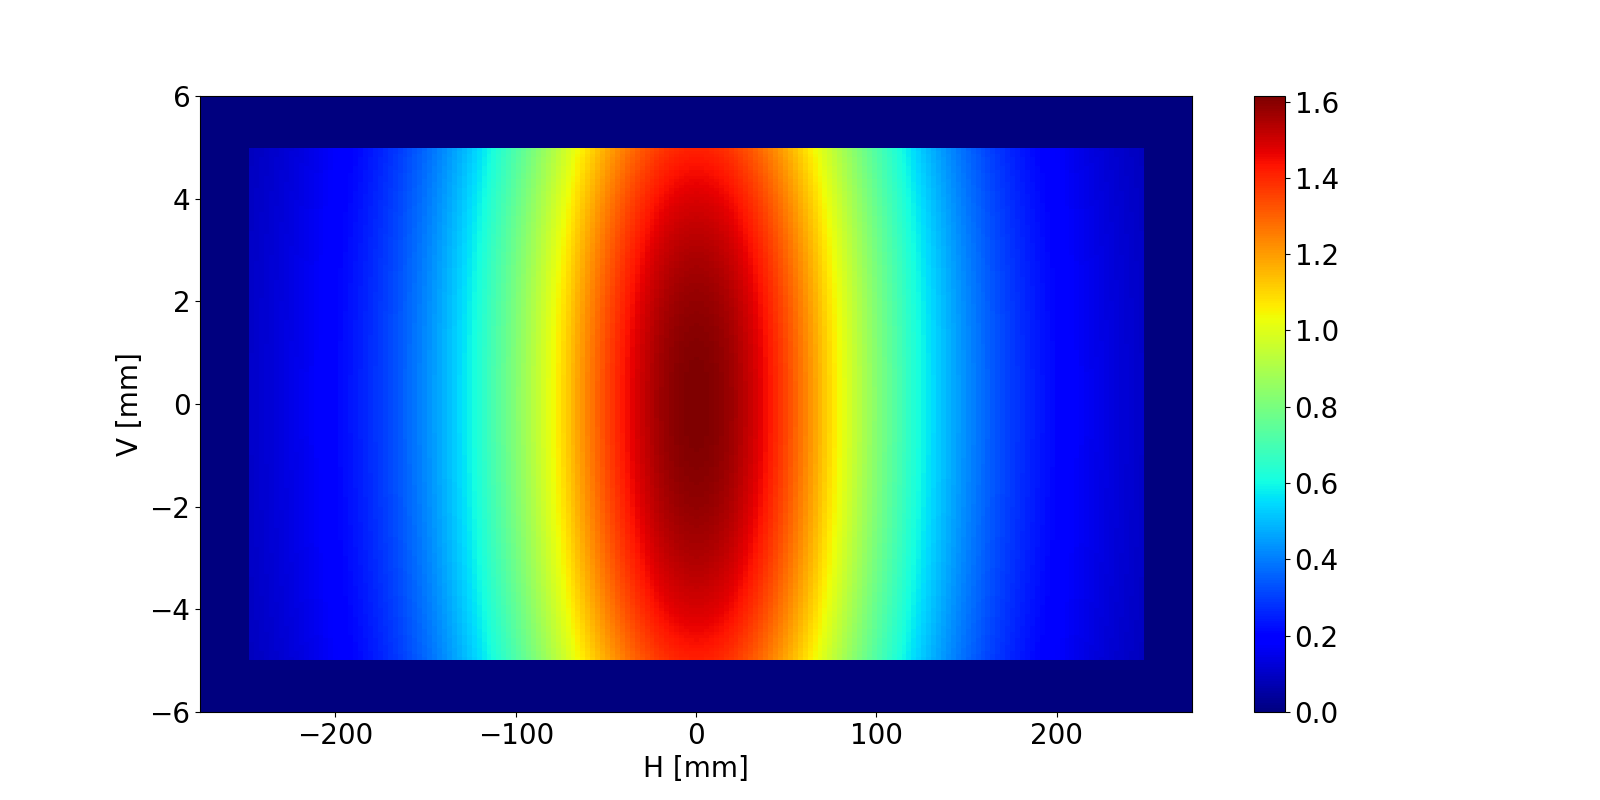
\includegraphics[width=0.45\textwidth]{figures/powerdensityKh.png}\\
%   c)~~~~~~~~~~~~~~~~~~~~~~~~~~~~~~~~~~~~~~~~~~~~
%   d)~~~~~~~~~~~~~~~~~~~~~~~~~~~~~~~~~~~~~~~~~~~~\\
%   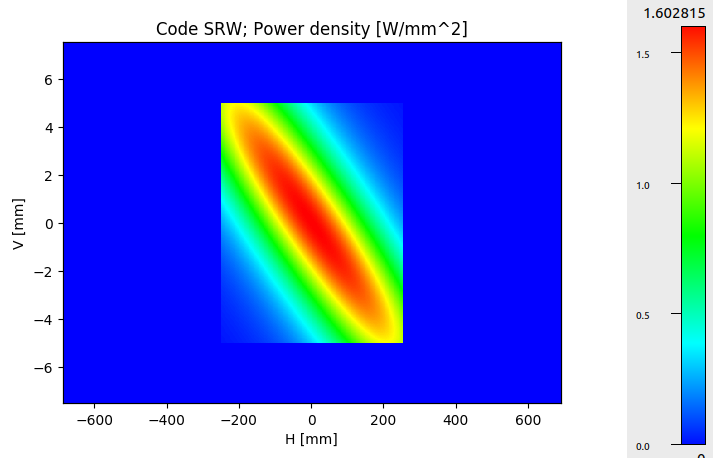
\includegraphics[width=0.45\textwidth]{figures/powerdensityKhKv.png} 
%      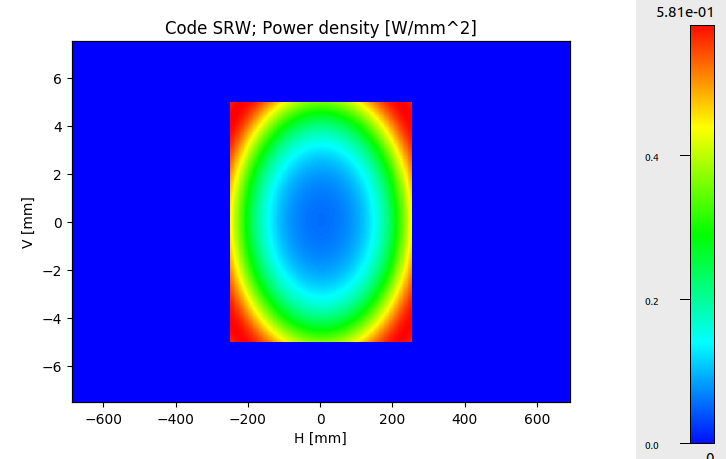
\includegraphics[width=0.45\textwidth]{figures/powerdensityKhKv90.png}
%\end{tabular}
%\end{center}
   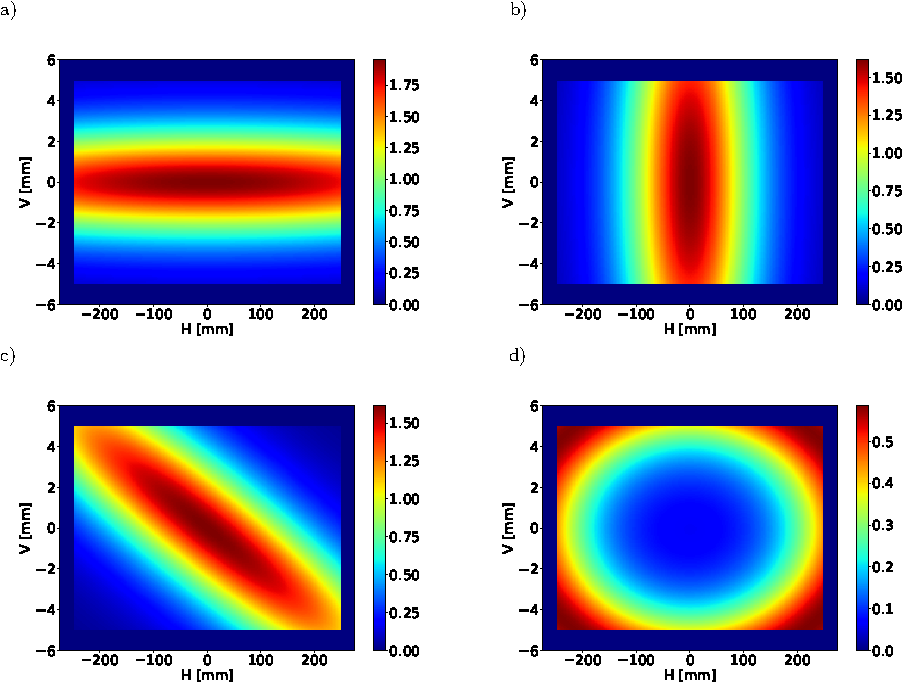
\includegraphics[width=1.0\textwidth]{figures/fig1.pdf} 
\caption
{Power density (in W/mm$^2$) on mirror M1.
a) $K_h=3.07, K_v=0$ (integrated power 3,523 W),
b) $K_h=0,K_v=3.07$ (integrated power 3,776 W),
c) $K_h=2.171,K_v=2.171, \Phi=0$ \textdegree (integrated power 3,978 W),
d) $K_h=2.171,K_v=2.171, \Phi=90$ \textdegree (integrated power 1,353 W).
}
\end{figure} 

In order to calculate the absorbed power density at the mirror, it is necessary to apply the energy-dependent mirror reflectance on the power density for different energies. There are several codes that can be used to compute this, e.g. SPECTRA \cite{codeSPECTRA}, SRCALC-IDPOWER \cite{SRCALC} and XOPPY. The last two are available in the OASYS environment. Table~\ref{tab:powerValues} shows the results in terms of power absorbed and peak power density as calculated by these three codes. 
\begin{table}\label{tab:powerValues}
    \caption{Absorbed power by the mirror M1 for two apertures with mirror illuminated areas of 460 $\times$ 10 mm$^2$ and 100 $\times$ 24 mm$&^2$  (6$\sigma$) as calculated by different codes. \inblue{The maximum photon energy considered for SRCALC and XOPPY calculations is 12 keV  .}

    }
    \resizebox{\textwidth}{!}{
    \begin{tabular}{lccc}
H polarization & SPECTRA & SRCALC & XOPPY \\
Power (W) in 460$\times$10 mm$^2$ & 
2070 & 
\inblue{2128} & 
2101 \\
Power (W) in 100$\times$2.4 mm$^2$ & 
239 & 
\inblue{247} & 
225 \\
Peak power density (W/mm$^2$) & 
1.01 & 
\inblue{1.13} & 
1.04  \\
\hline\hline
V polarization & SPECTRA & SRCALC & XOPPY \\
Power (W) in 460$\times$10 mm$^2$ &
2070 & 
\inblue{2122} & 
2126   \\
Power (W) in 100$\times$2.4 mm$^2$ & 
216 & 
\inblue{249} & 
227 \\
Peak power density (W/mm$^2$) & 
1.01 & 
\inblue{1.12} & 
1.05  \\
% \hline\hline
% Circ polarization & SPECTRA & SRCALC & XOPPY \\
% Power (W) in 500$\times$10 mm$^2$ & 
% - & 
% 535 (42.6\%) & 
% 404.2 (37.3\%)     \\
% Power (W) in 100$\times$2.4 mm$^2$ & 
% - & 
% 3.30 (21.3\%) & 
% 1.43 (21.2\%)     \\
% Peak power density (W/mm$^2$) & 
% - & 
% 0.42 & 
% 0.04     \\

    \end{tabular}
    }
\end{table}

\subsection{Deformation of M1 due to heat load}

The distortion of the mirror was calculated using the finite-element method (FEM), as implemented in ANSYS software (\url{http://ansys.com}) for the horizontal and vertical polarizations. The case of circular polarizations has not been considered because of the small absorbed power. The FEM calculation generates a map of the surface deformation for a given heat load and mirror design, including cooling. Figure~\ref{fig:M1deformation} shows the deformation maps (column 1) and the tangential profile at the mirror center (column 2). The maps were loaded in OASYS using a dedicated widget that also extracts the 1D profile and for the reflector widget.

We calculated surface deformations for two different cooling schemes: a water-side-cooled mirror and a liquid-nitrogen-cooled mirror \cite{cutler}. Both mirrors are made from single-crystal silicon substrates.
The liquid-nitrogen-cooled mirror substrate has a trapezoidal shape. In the case of the water-side-cooled mirror, we controlled distortion by a combination of mirror design parameters, including beam overfilling, a notched or smart-cut substrate, and tuned cooling length \cite{Zhang}. Note that we did not optimize these parameters to minimize height or slope error, but instead chose parameters for a range of heat loads, and to facilitate adaptive correction.

It is important to note that our water-cooled finite element model does not include a mounting or cooling system, and therefore the presented results should be seen as a `best' or idealized case.  In other words, the shape of an actual water-cooled mirror will be more difficult to correct than what the calculations in this model indicate. In contrast, our model of the liquid-nitrogen-cooled mirror does includes mounting and cooling system deformation, and therefore is a more realistic model than what is presented for the water-side-cooled case.

  \begin{figure}
  \label{fig:M1deformation} 
%  \begin{center}
%   \begin{tabular}{l} 
%   a$_1$)~~~~~~~~~~~~~~~~~~~~~~~~~~~~~
%   a$_2$)~~~~~~~~~~~~~~~~~~~~~~~~~~~~~a$_3$)\\
%   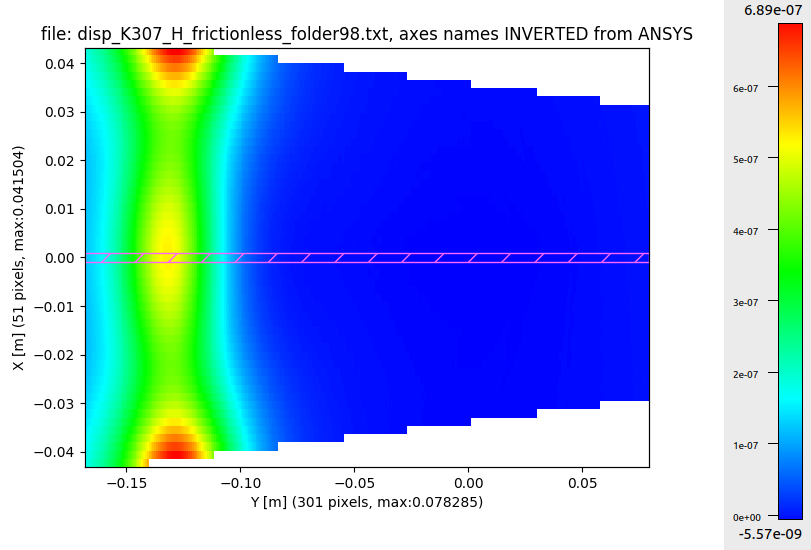
\includegraphics[width=0.32\textwidth]{figures/cryogenic2d.png} 
%   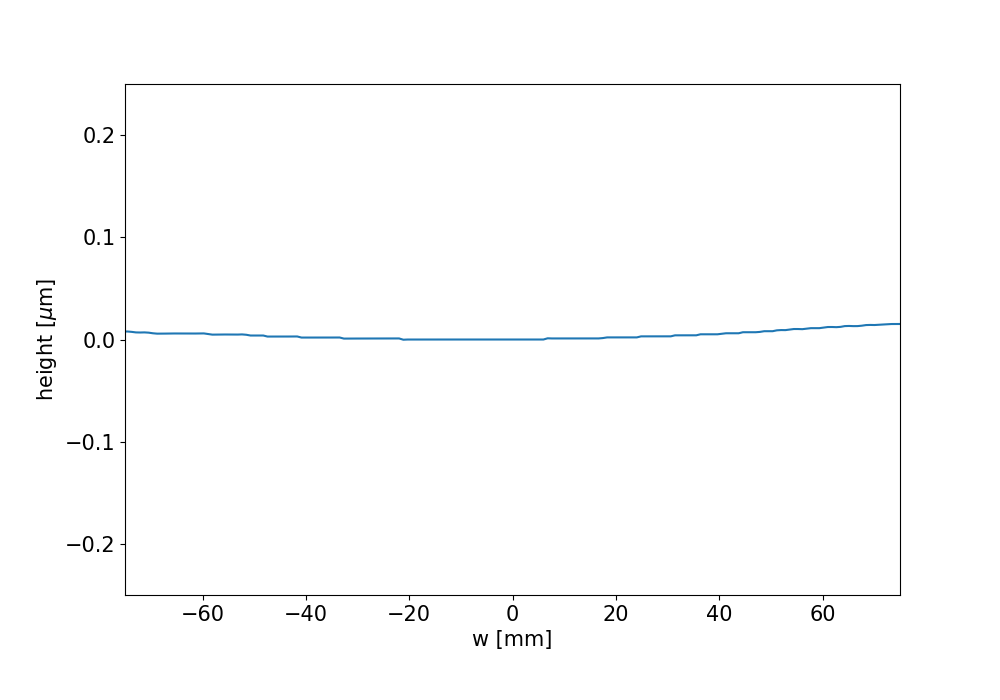
\includegraphics[width=0.32\textwidth]{figures/deformation1.png}
%   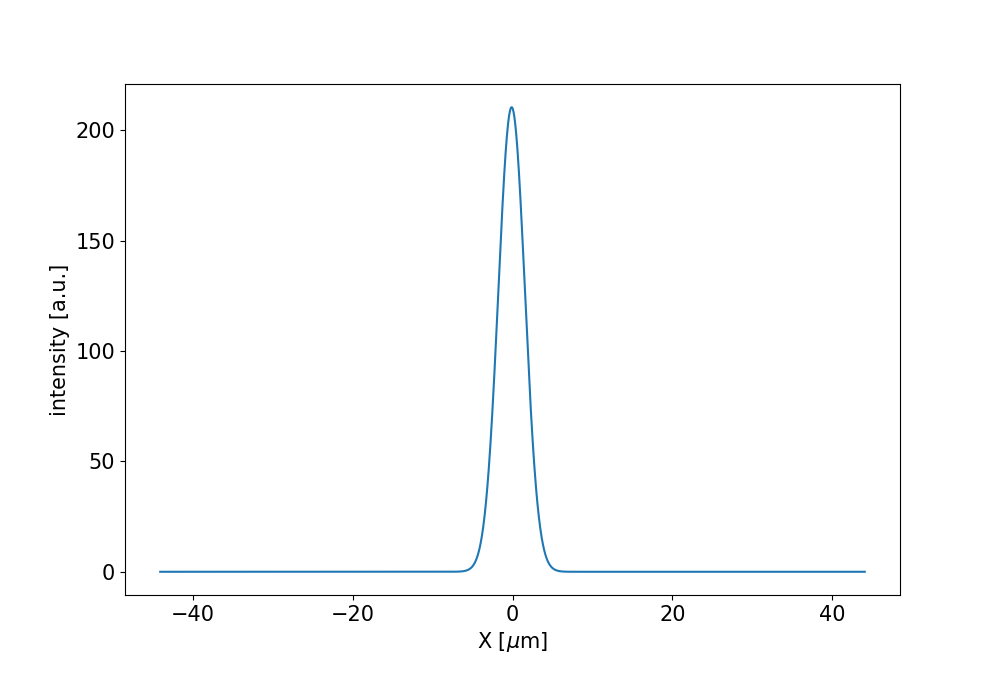
\includegraphics[width=0.32\textwidth]{figures/intensity1.png} \\
%
%  b$_1$)~~~~~~~~~~~~~~~~~~~~~~~~~~~~~
%  b$_2$)~~~~~~~~~~~~~~~~~~~~~~~~~~~~~b$_3$)\\
%  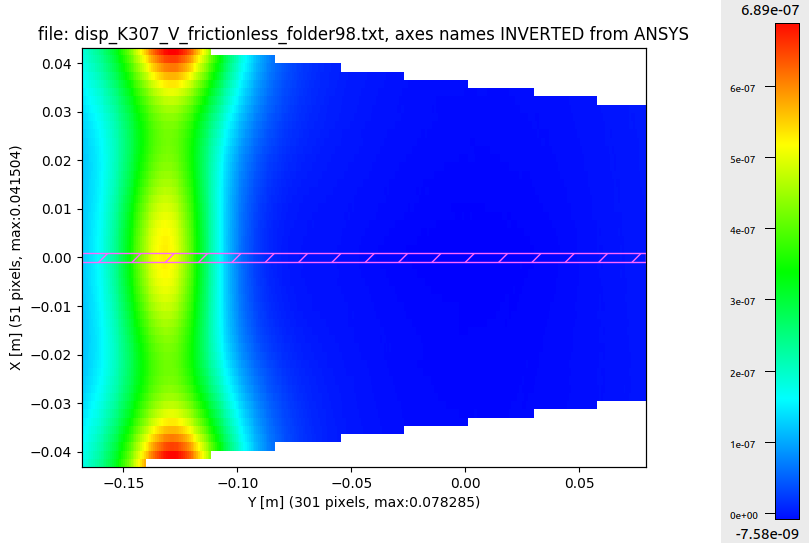
\includegraphics[width=0.32\textwidth]{figures/cryogenic2dKh.png}
%  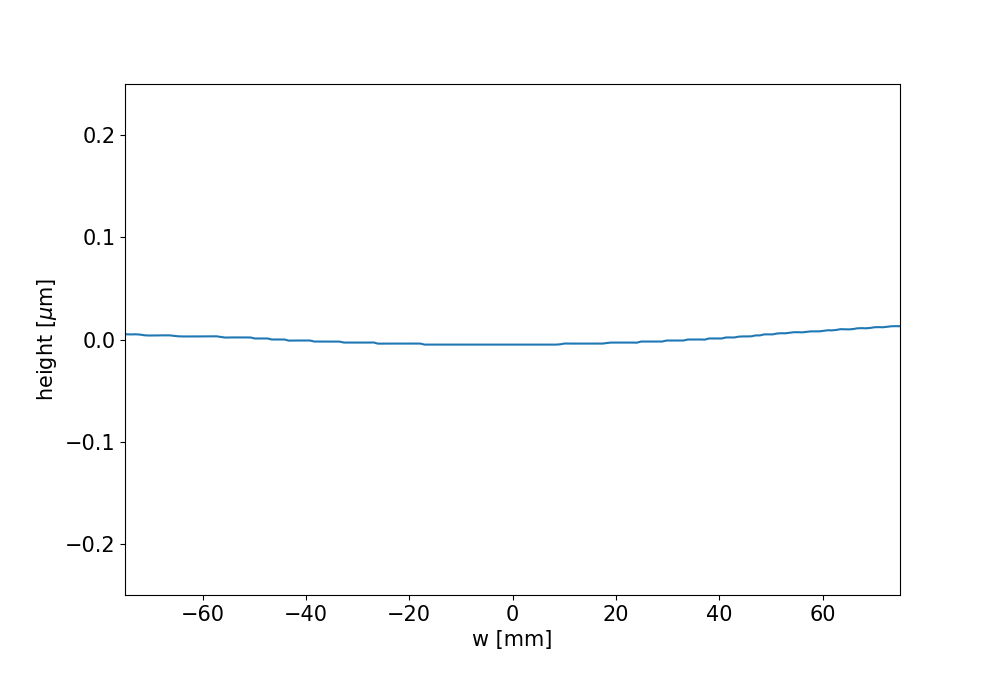
\includegraphics[width=0.32\textwidth]{figures/deformation2.png}
%  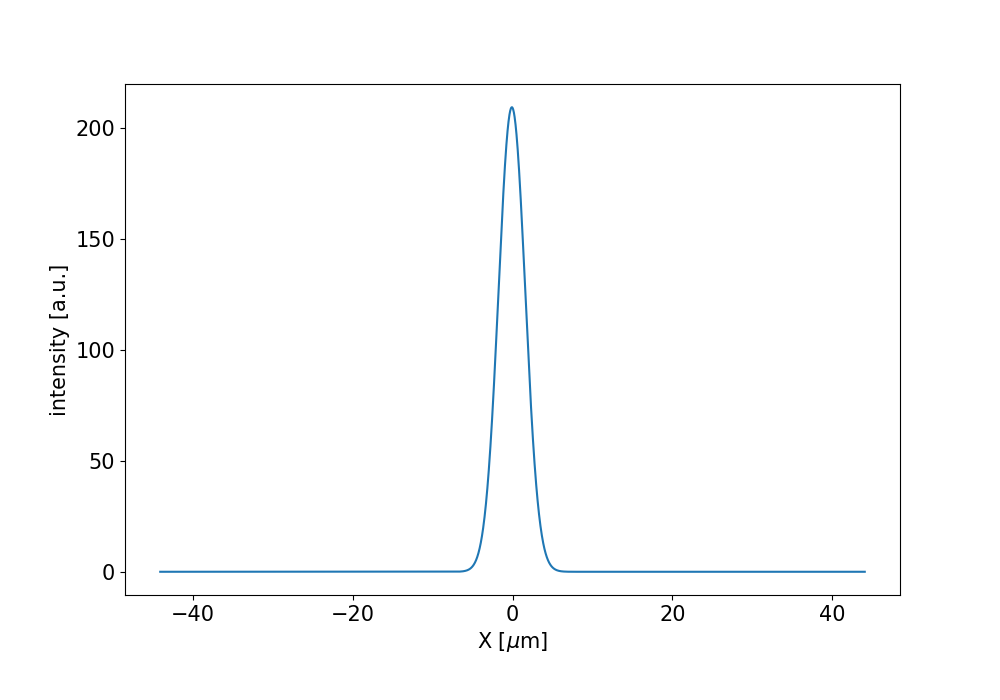
\includegraphics[width=0.32\textwidth]{figures/intensity2.png} \\
%   
%   c$_1$)~~~~~~~~~~~~~~~~~~~~~~~~~~~~~
%   c$_2$)~~~~~~~~~~~~~~~~~~~~~~~~~~~~~c$_3$)\\ 
%   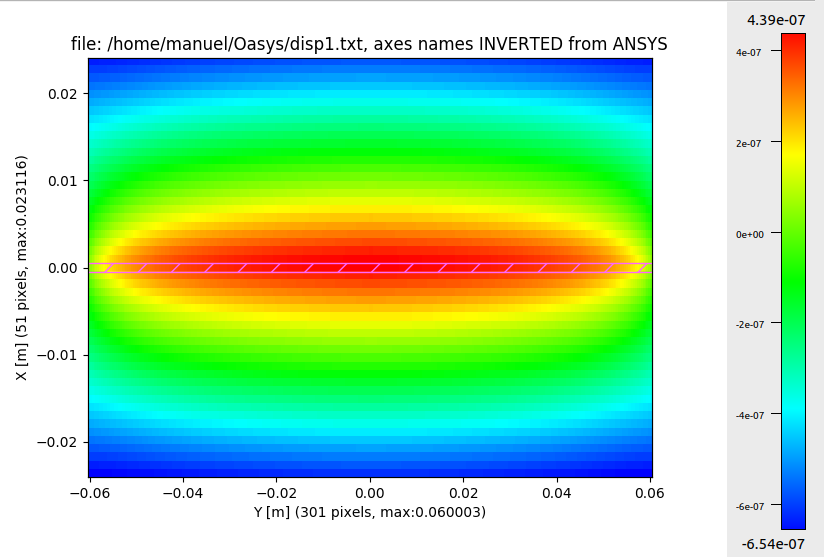
\includegraphics[width=0.32\textwidth]{figures/water1_2d.png}
%   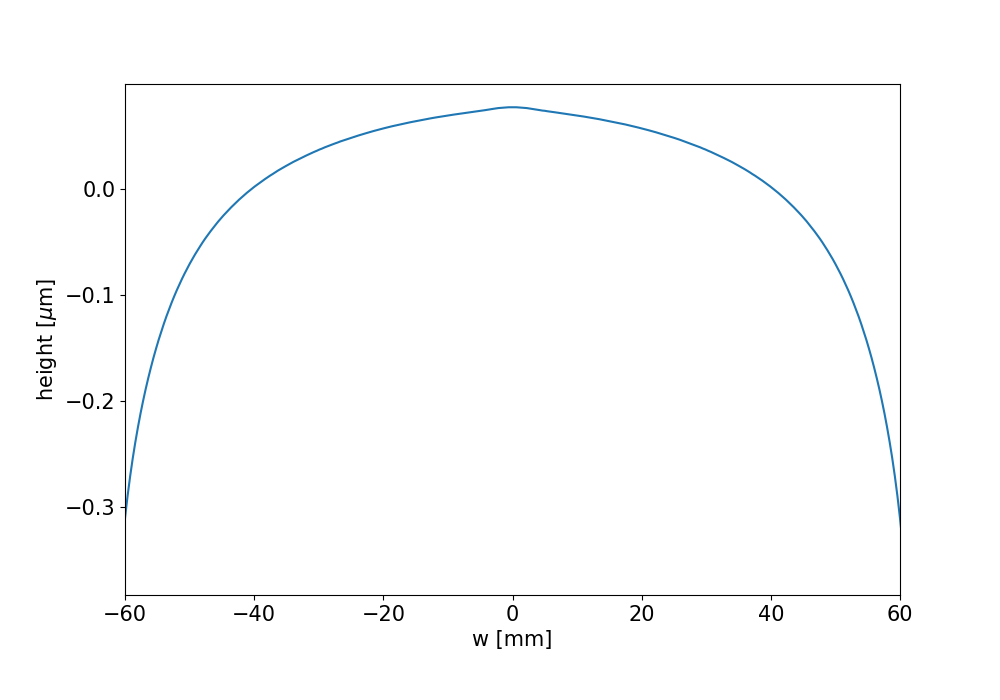
\includegraphics[width=0.32\textwidth]{figures/deformation3.png}   
%   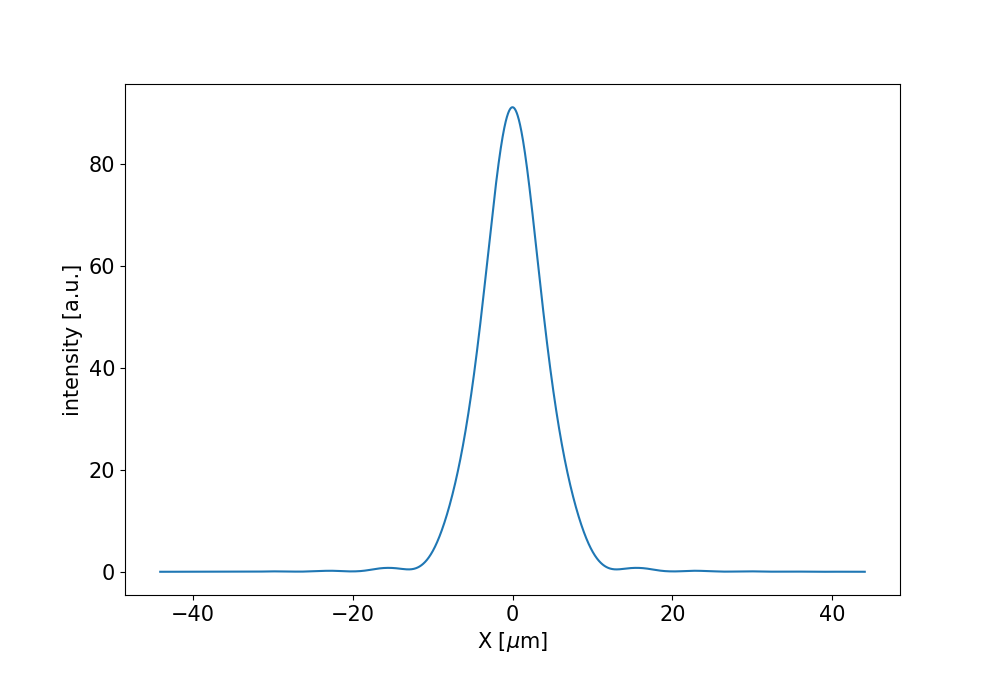
\includegraphics[width=0.32\textwidth]{figures/intensity3.png} \\
%
%   
%   d$_1$)~~~~~~~~~~~~~~~~~~~~~~~~~~~~~
%   d$_2$)~~~~~~~~~~~~~~~~~~~~~~~~~~~~~d$_3$)\\
%   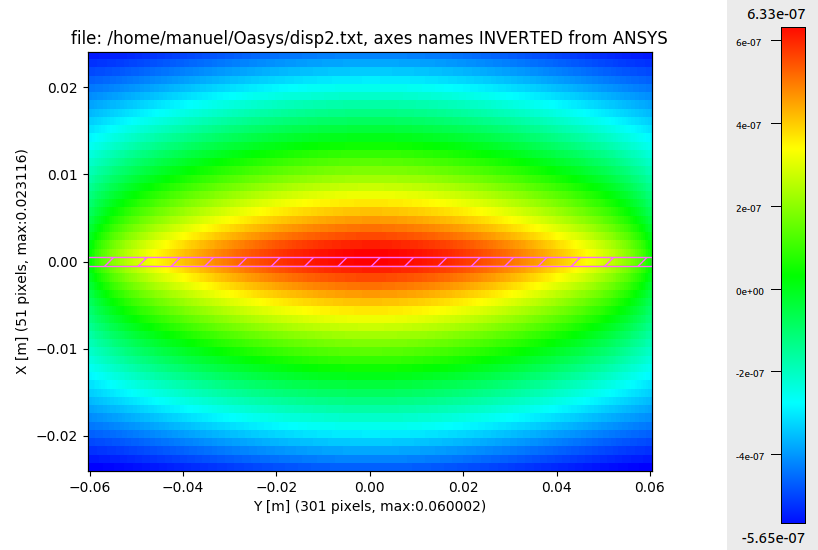
\includegraphics[width=0.32\textwidth]{figures/water2_2d.png} 
%   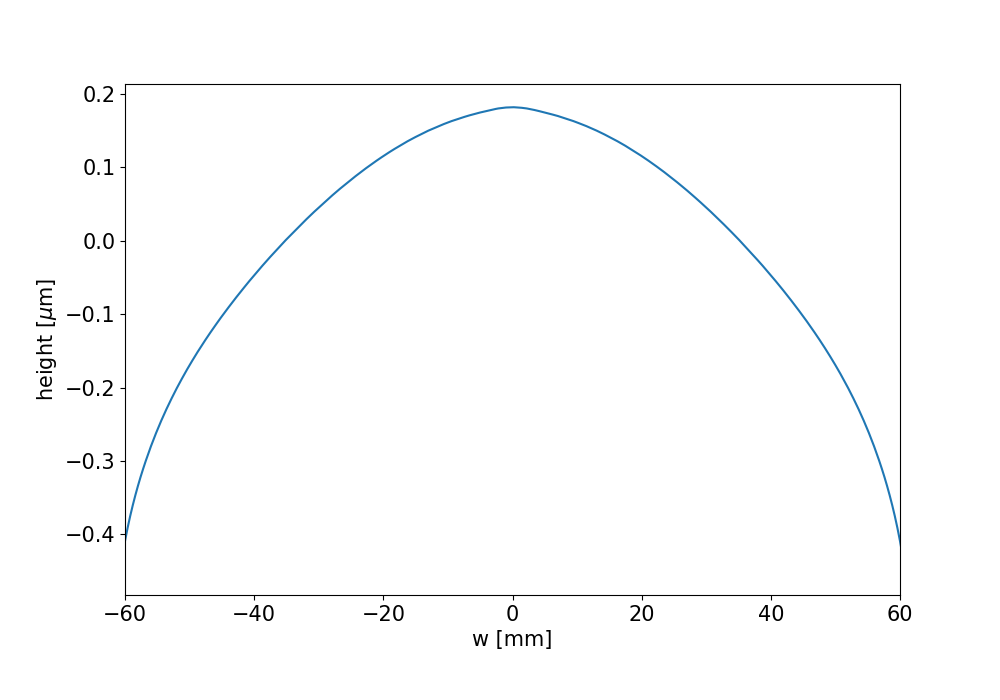
\includegraphics[width=0.32\textwidth]{figures/deformation4.png} 
%   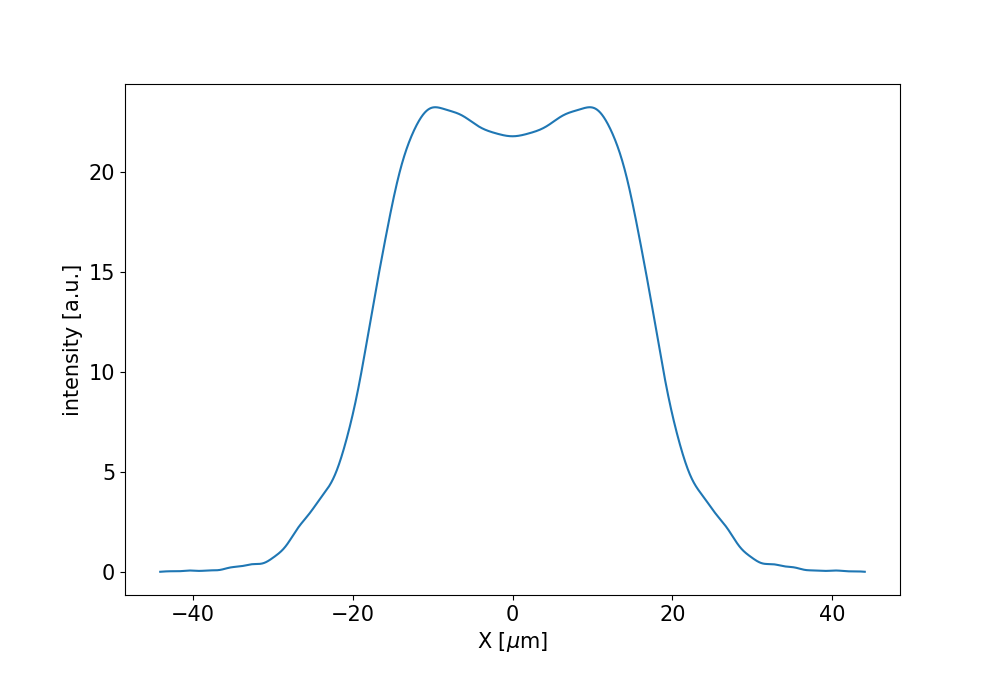
\includegraphics[width=0.32\textwidth]{figures/intensity4.png}\\
%   
%   \end{tabular}
%  \end{center}
   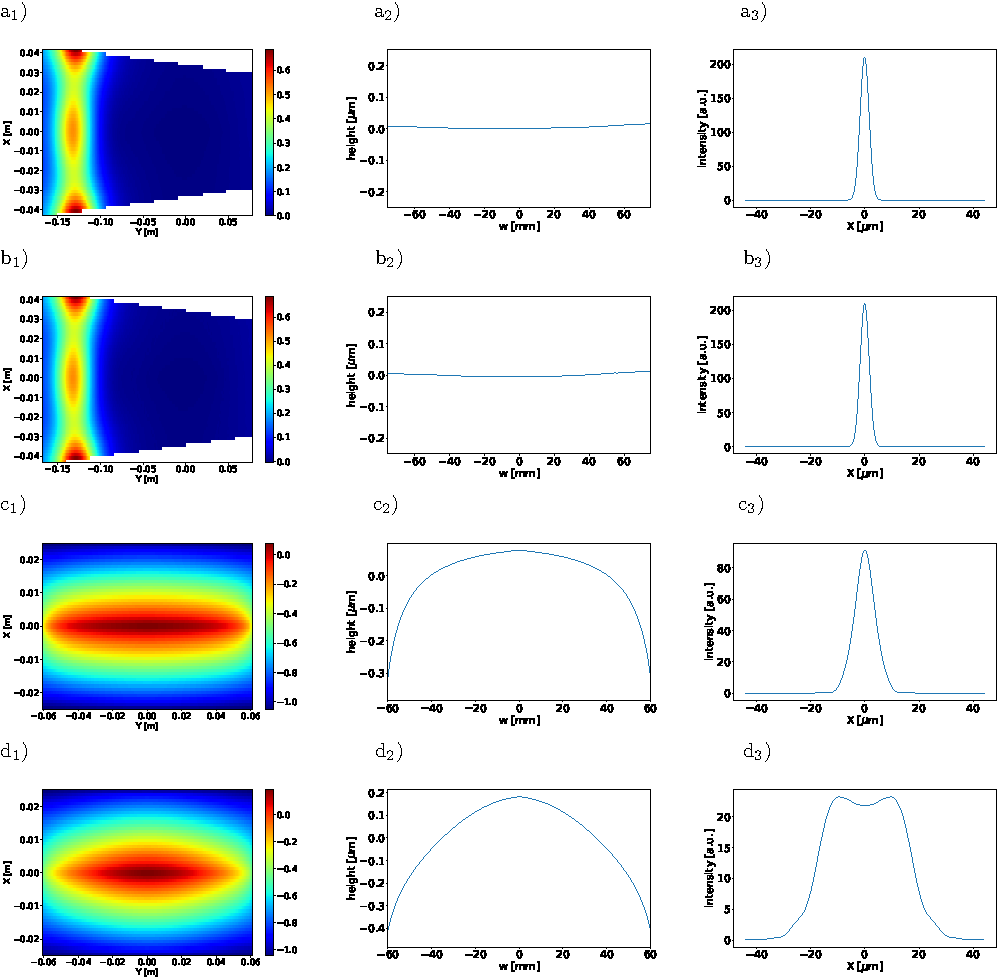
\includegraphics[width=1.0\textwidth]{figures/fig2.pdf}
   \caption
   { 
   Left column: 2D map of the surface deformation: a$_1$) cryogenic mirror for $K_h=3.07$, $K_v=0$; b$_1$) cryogenic mirror for $K_h=0$, $K_v=3.07$; c$_1$) water-cooled mirror $K_h=3.07$, $K_v=0$; d$_1$) water-cooled mirror $K_h=0$, $K_v=3.07$. Central column: the extracted 1D profiles a$_2$,b$_2$,c$_2$, and d$_2$ respectively. Right column: The focused image with these profiles are in Figs.~a$_3$, b$_3$, c$_3$ and d$_3$, respectively. 
   The FWHM values are: 3.85, 3.91, 8.53 and 36.34 $\mu$m, respectively (3.68 $\mu$m for the undeformed one) and the Strehl ratios: 0.99, 0.98, 0.43 and 0.11, respectively (one for the undeformed mirror).
   }
   \end{figure} 


\subsection{Beamline simulation and effect of uncorrected M1 deformation}

The beamline simulation has been performed using WOFRY using the algorithms described in section~\ref{sec:wofry}. The undulator field is calculated at a position just before M1 ($y$=13.73 m) using the model described in section~\ref{sec:undulator}. M1 is a plane reflector that can be deformed in the model, using a given deformation profile. We began with no deformation. The wavefront is propagated through free space from M1 to M3 at a distance of 13.599 m, using the zoom propagator (section~\ref{sec:zoomPropagator}). Then M3 is treated as an ideal reflector with a radius $R=220.72$~m obtained from the lens equation $1/p + 1/q=1/f=2/R \sin \theta$ with $p$=13.73+13.599~m, $q$=2.64~m, $\theta$=1.25~\textdegree. With no M1 deformation, the image has a full-width at half maximum of 3.84~$\mu$m (Fig.~\ref{fig:nodeformation} and an intensity of 213 in arbitrary units; this value will be used to normalize intensities with the non-deformed case and calculate the Strehl ratio.

\begin{figure} 
\label{fig:nodeformation} 
\begin{center}
\begin{tabular}{c} 
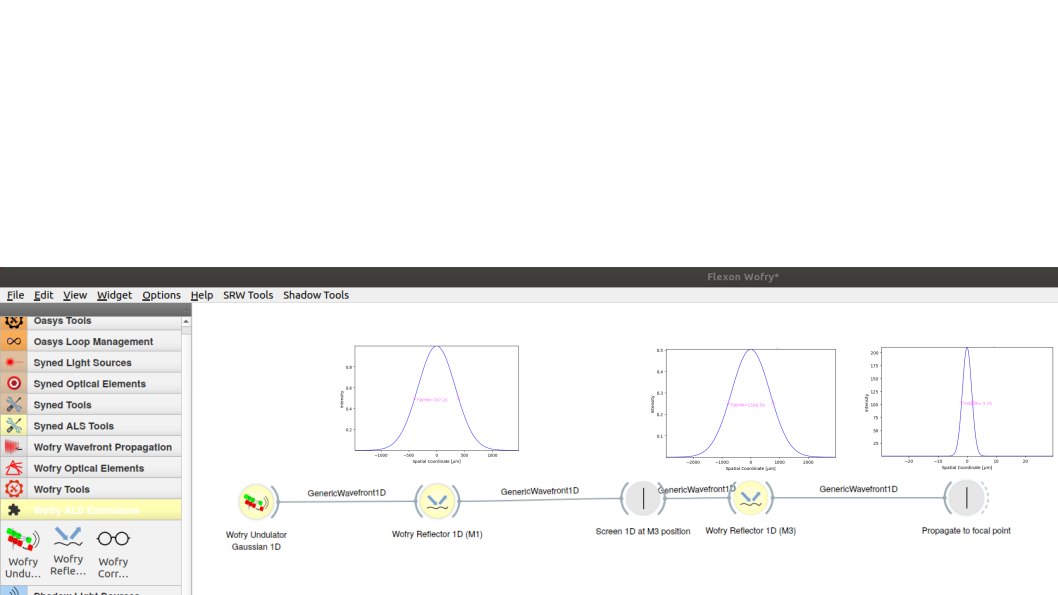
\includegraphics[width=0.95\textwidth]{figures/wofrynodeformation.png}
\end{tabular}
\end{center}
\caption{ 
OASYS workspace showing the simulation for the beamline with no deformation in M1. The intensity profile of the beam are superposed at different positions, with FWHM of 819~$\mu$m at M1, 1,631~$\mu$m at M3 and 3.82~$\mu$m at the focal position.  }
\end{figure} 

We can evaluate the focusing properties using two commonly applied metrics: the full-width at half-maximum (FWHM) and the Strehl ratio \cite{Strehl}. The Strehl ratio compares the peak intensity at focus to the ideal value in a system free of aberrations. Applying the different M1 shape deformations, we find the following. For the cryogenically-cooled mirror, where the rms height error is about 4 nm, there is no significant reduction of the intensity distribution of the image; the FWHM increases slightly, from 3.82$\mu$m to 3.85$\mu$m with horizontal polarization, and to 3.91$\mu$m for vertical polarization. The Strehl ratio is reduced to 0.99 and 0.98 for the two polarizations, respectively (column 3 in Fig.~\ref{fig:M1deformation}). For the water-cooled mirror, where the rms height error is about 40~nm and 100~nm for horizontal and vertical polarizations, the degradation is more significant. The focal spot broadens to FWHM~=~8.53~$\mu$m and 36.34$\mu$m for the two polarizations, with a consequent Strehl ratio reduction to 0.43 (H) and 0.11 (V), values that are unacceptable for most applications. 

We can conclude that the cryogenic cooling is almost perfect in the sense that it does not alter the intensity distribution with optimum Strehl ratios. The deformation in the water cooled mirrors produces a large deterioration of the intensity profile for both cases of polarization. The associated Strehl ratio are far away from what is usually accepted (larger than 0.8, corresponding to Marechal criterion \cite{Marechal} ). There is a larger deterioration for the case of $K_v\ne 0$ corresponding to light polarized in the plane perpendicular to the electron orbit. The next section discusses whether the AXO can improve the situation for water-cooled mirrors.    

\subsection{Adaptive X-ray Optics M3. Ideal case.}

The M3 mirror is adaptive, fabricated with a predefined elliptical shape at rest. It incorporates a bimorph mechanism able to modify the ellipse in the tangential direction (horizontal), as necessary to compensate and correct wavefront errors. It will work with feedback from a wavefront sensor placed just downstream from it. The diagnostic system will analyze the wavefront phase and amplitude, calculate the distortion as a difference from the measured phase map and the ideal one, compute the correcting mirror profile, and calculate the inputs for the adaptive optics actuators required to achieve the desired profile, and also account for additional effects (back-end, dynamic effects).

To simulate the AXO, an OASYS widget ``WOFRY corrector (reflector)'' computes and applies the correction to the wavefront in the following way: i) it extracts the phase from the incident wave $\phi_{inc}(x)$, ii)  it calculates the phase of the spherical wave collapsing to this focal position $\phi_{sph}(x)$, given a distance to focus, %the waist (position where we want to focus), 
iii) it calculates the phase difference $\Delta \phi(x) = \phi_{sph} - \phi_{inc}$, and iv) it computes the profile height $h(w) = -\Delta \phi(w) / (2 k \sin \theta)$. In this model we extract the phase of the wavefront and calculate the corrective profile deterministically, comparing this phase with the spherical collapsing wave without weighting the resulting profile. It should be mentioned that this method could be improved by doing an optimization of the profile to maximize the Strehl ratio, a process where the weight applied to the profile plays a fundamental role \cite{Goldberg2016}.

   \begin{figure}
   \label{fig:intensitycorrected} 
%   \begin{center}
%   \begin{tabular}{l}
%  a$_1$)~~~~~~~~~~~~~~~~~~~~~~~~~~~~~~~~~
%  a$_2$)\\
%    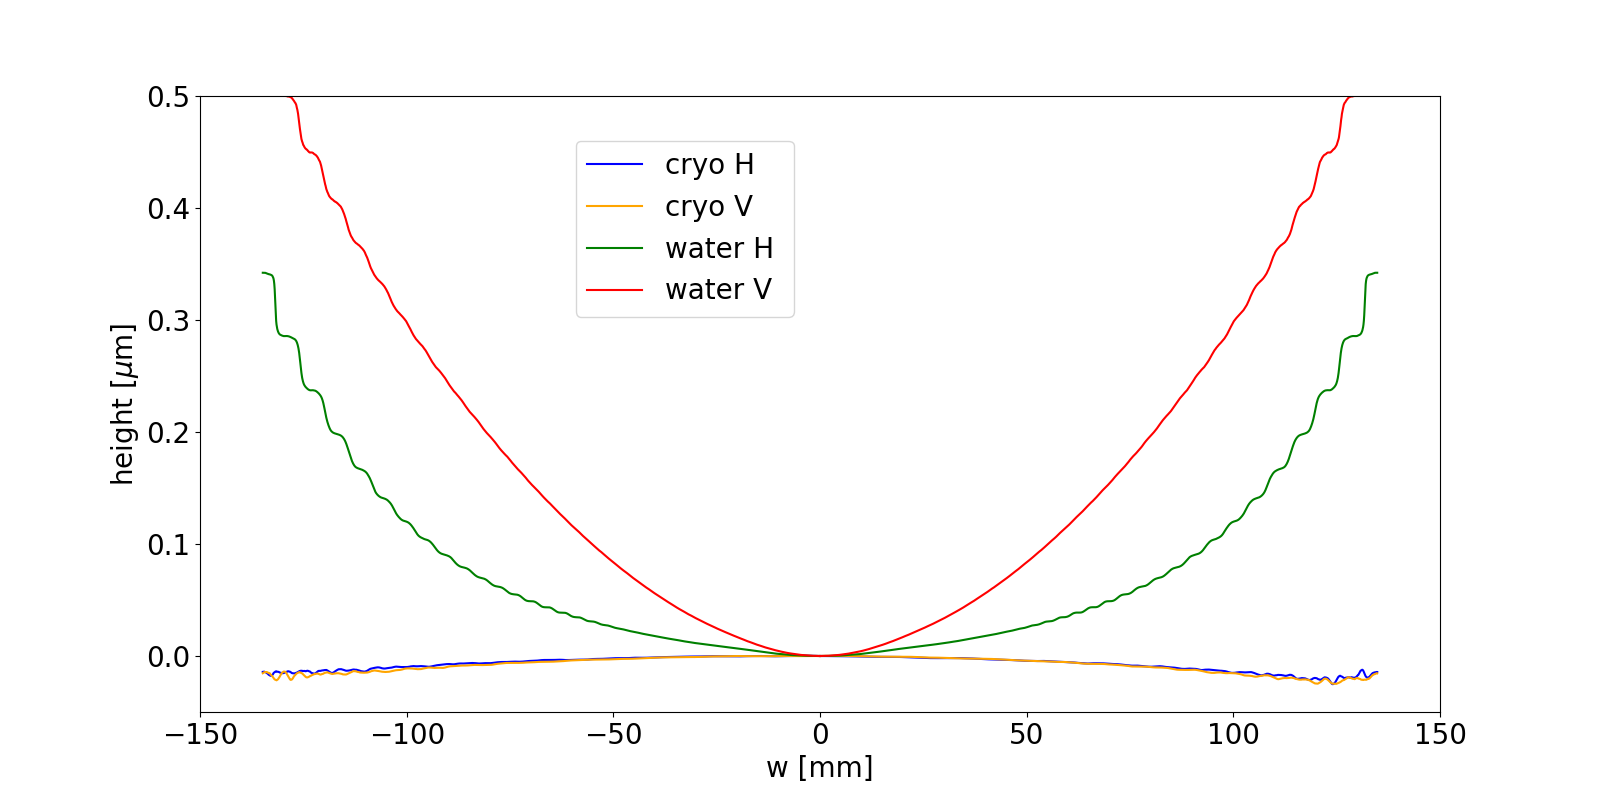
\includegraphics[width=0.5\textwidth]{figures/correctionprofiles.png}
%    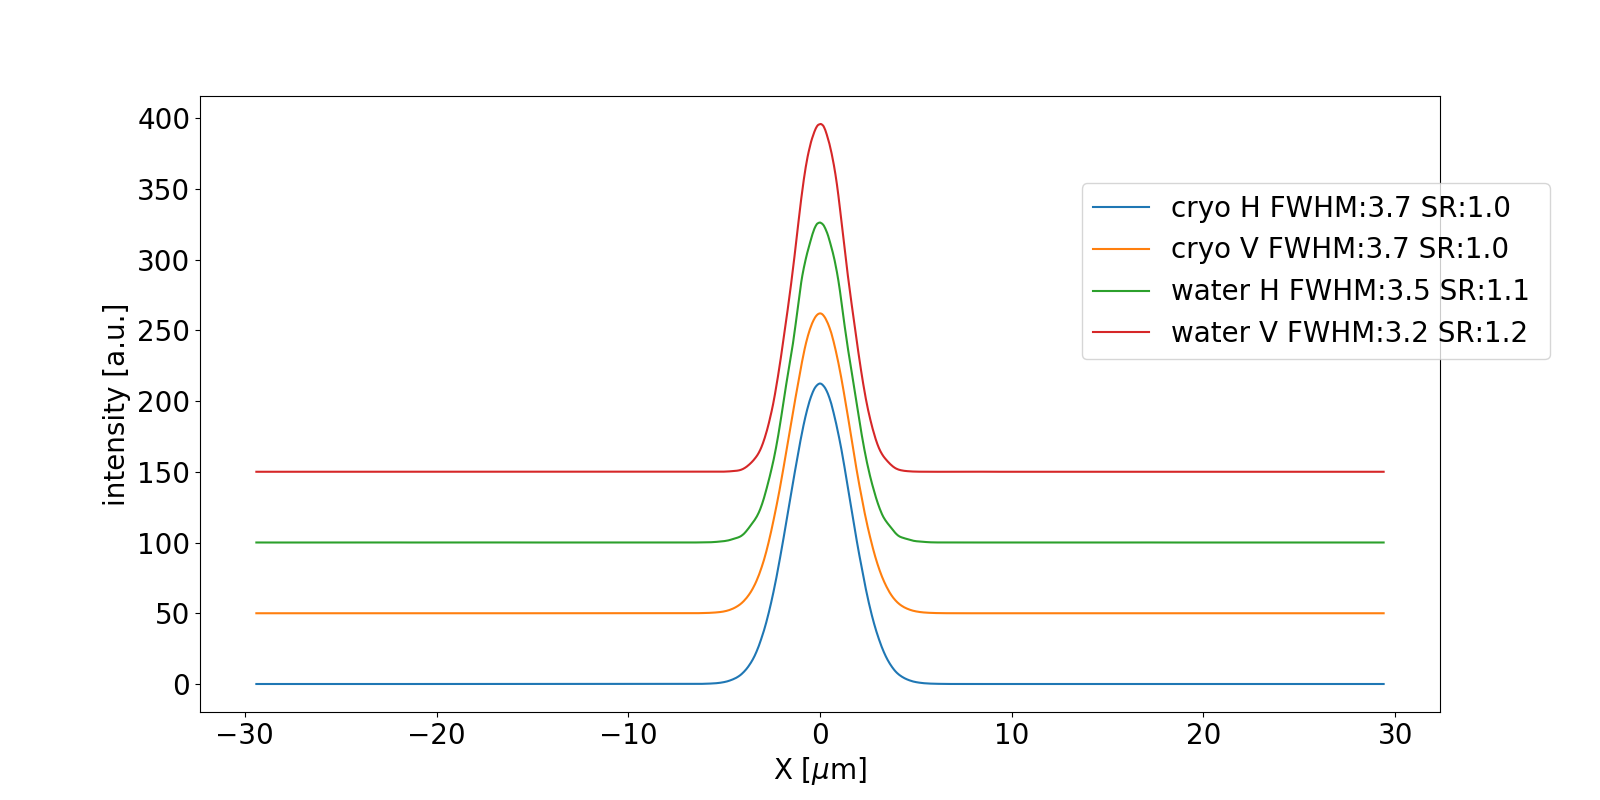
\includegraphics[width=0.5\textwidth]{figures/intensitycorrected.png} \\
%  b$_1$)~~~~~~~~~~~~~~~~~~~~~~~~~~~~~~~~~
%  b$_2$)\\
%   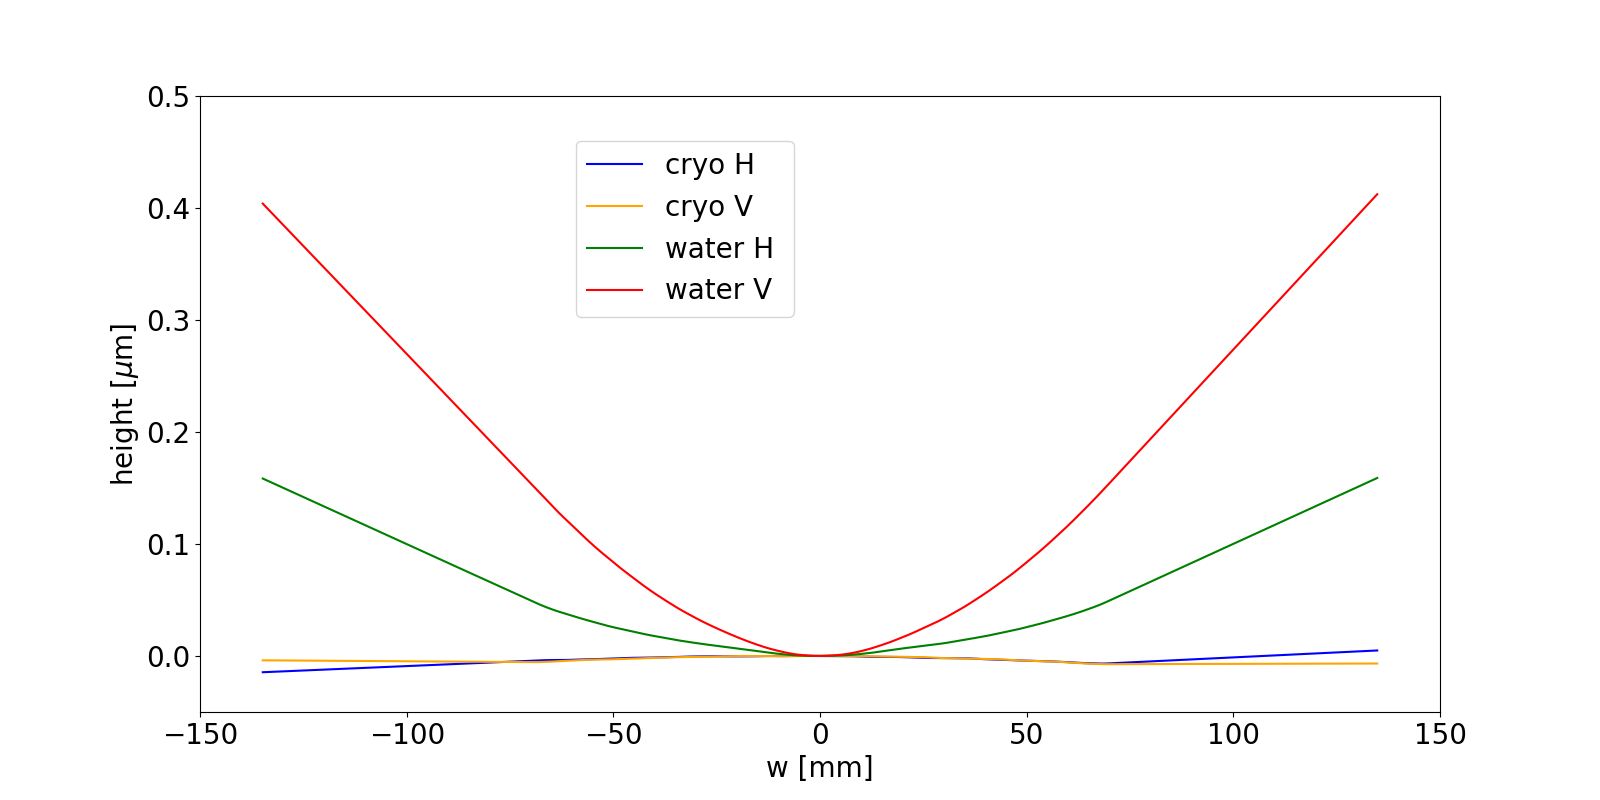
\includegraphics[width=0.5\textwidth]{figures/correctionprofilesextrapolated.png}
%   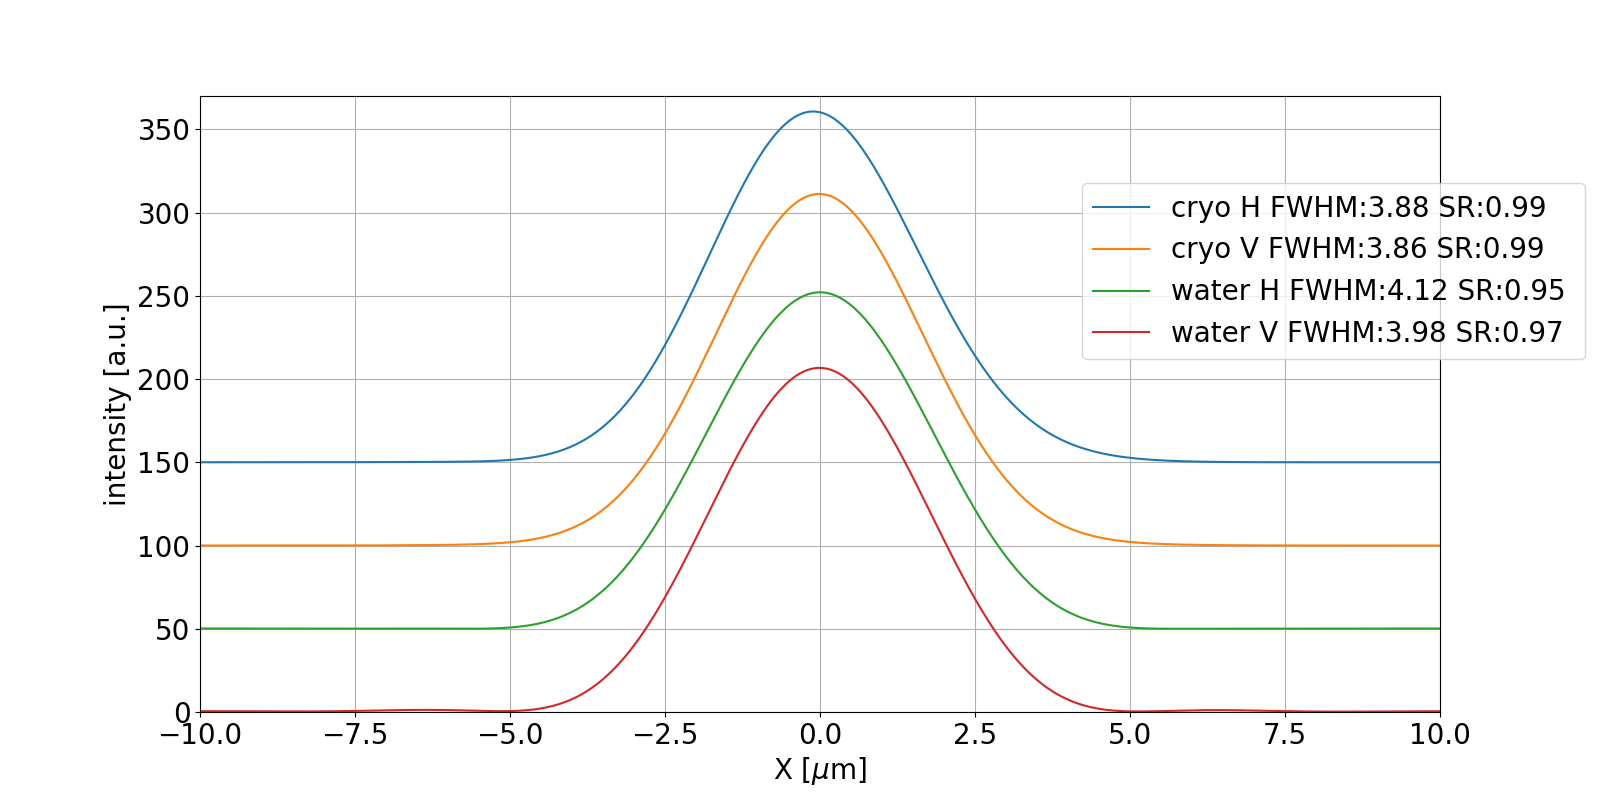
\includegraphics[width=0.5\textwidth]{figures/intensitycorrectedextrapolated.png} \\
%  c$_1$)~~~~~~~~~~~~~~~~~~~~~~~~~~~~~~~~~
%  c$_2$)\\
%   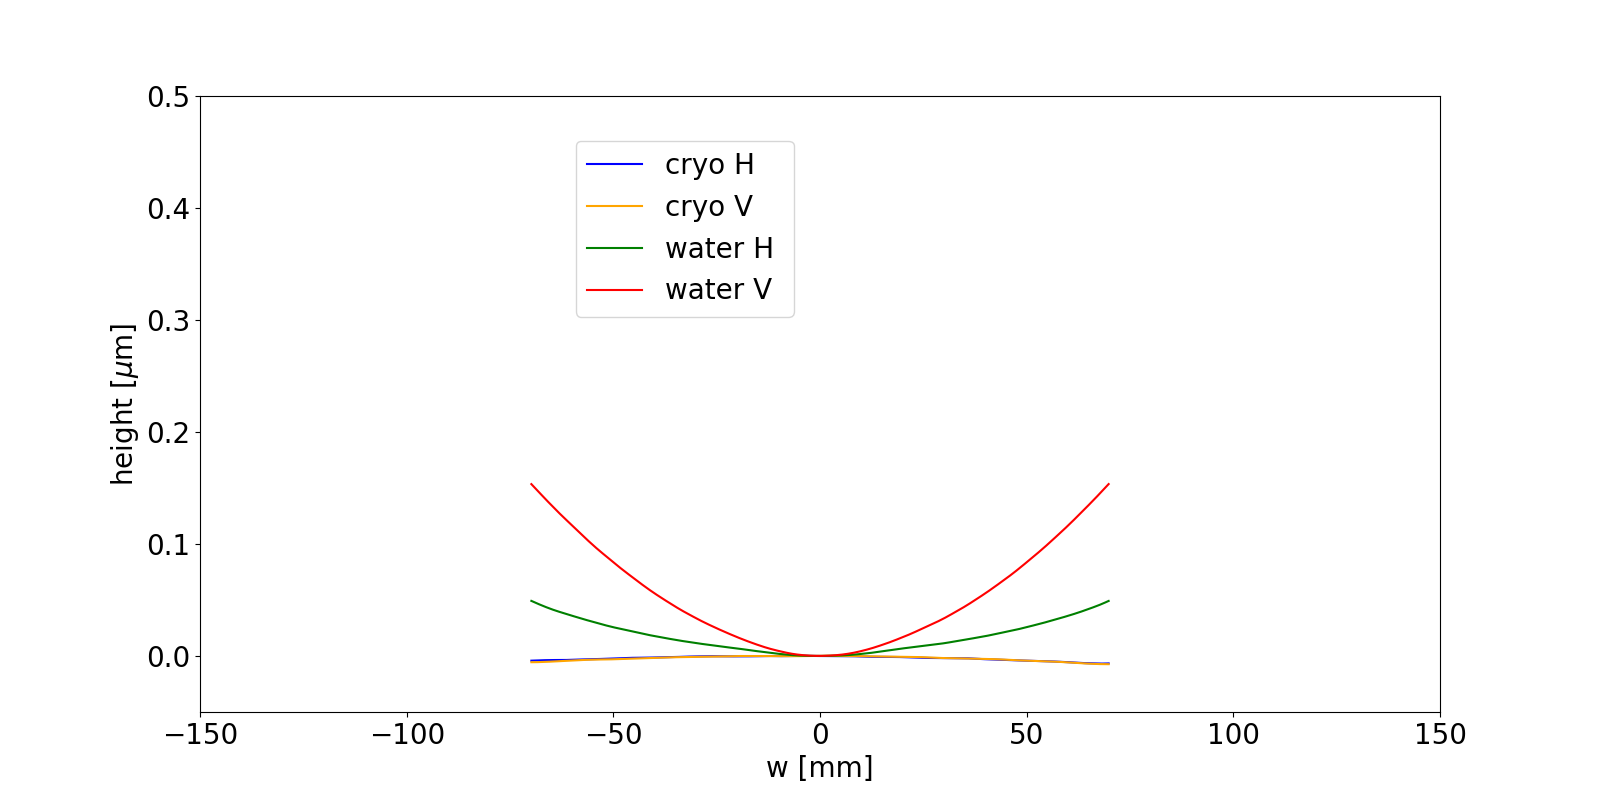
\includegraphics[width=0.5\textwidth]{figures/correctionprofilescropped.png}
%   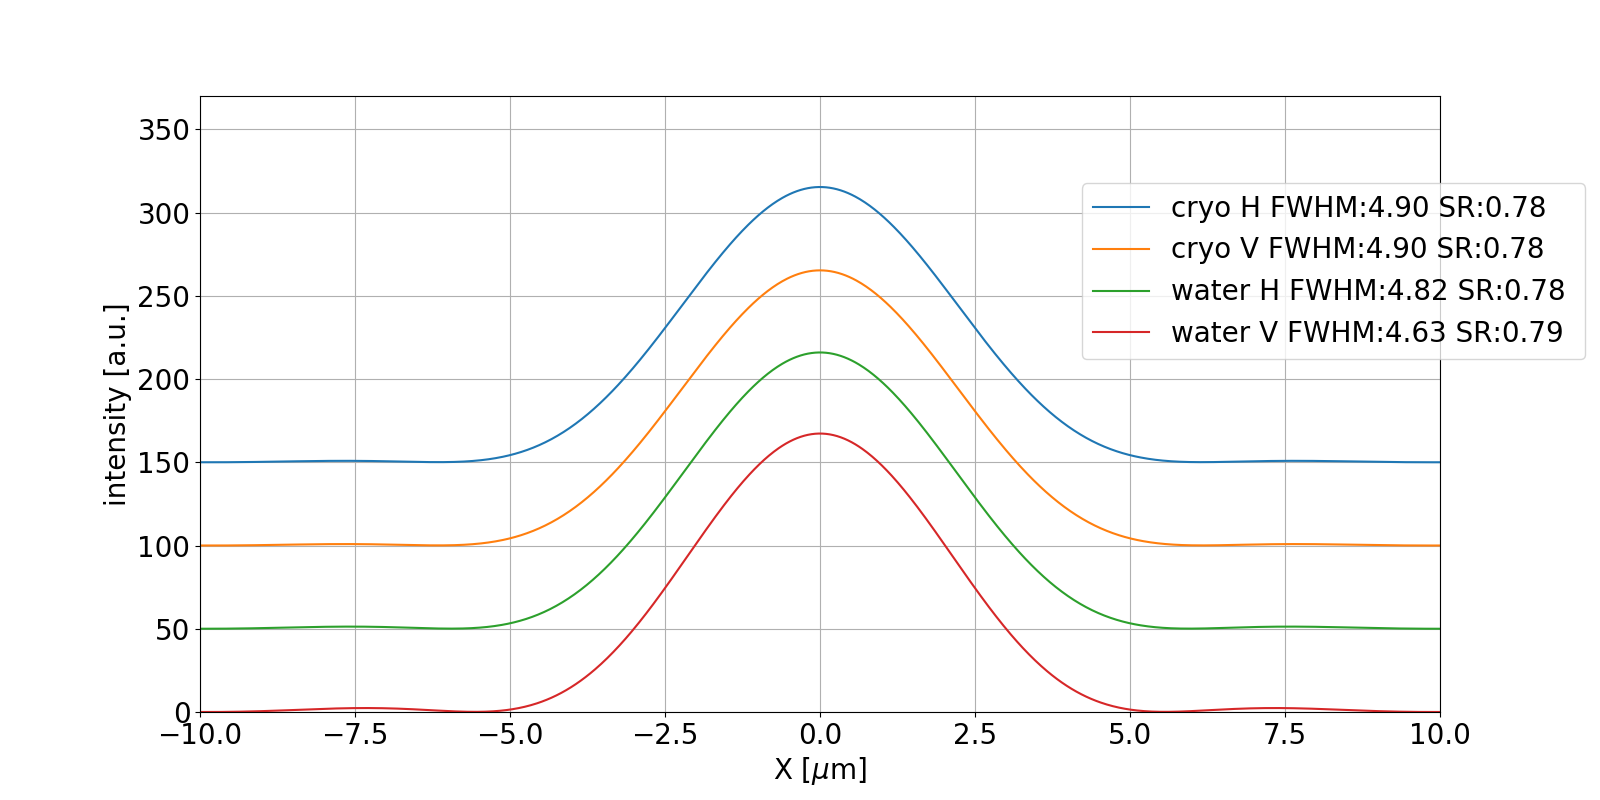
\includegraphics[width=0.5\textwidth]{figures/intensitycorrectedcropped.png}\\
%   \end{tabular}
%   \end{center}
   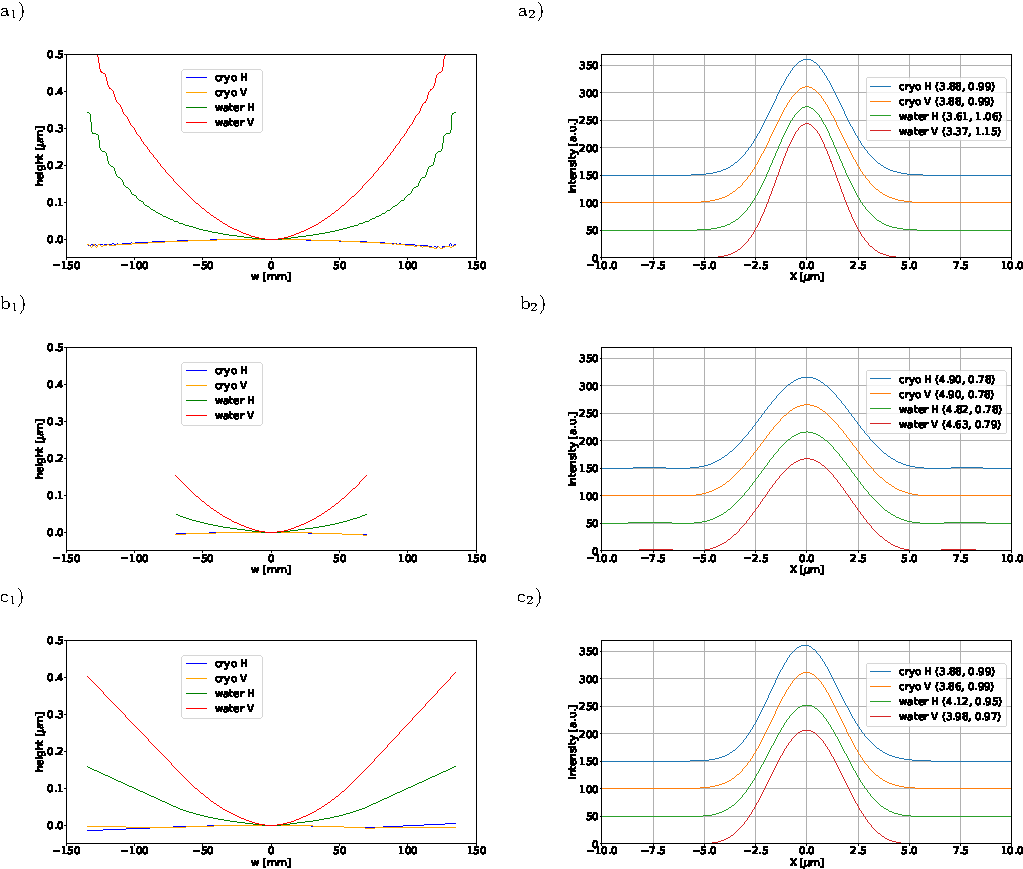
\includegraphics[width=1.0\textwidth]{figures/fig4.pdf}\\
   \caption
   { Correction profile on M3 (left) and intensity distribution (right) at the focal position when the different deformations of M1 are corrected by the AXO in M3 using  a) ideal correction profile, b) expansion of the ideal profiles as a function of the AXO orthonormal basis which defines a shorter mirror, and c) \inblue{expansion of the ideal profiles as a function of the AXO orthonormal basis and then making a linear extrapolation at the edges to the longer mirror length}. Note that the intensity profiles have been shifted vertically for clarity. }
   \end{figure} 


Fig.~\ref{fig:intensitycorrected}a shows the result using the corrected profiles added to the elliptical shape of the mirror. We observe that the correction results in an intensity distribution and Strehl ratio that are very close to the case using the ideal, undeformed M1. The Strehl ratio has been calculated as the ratio of the peak intensity for the deformed M1 and corrected M3 mirrors over the peak intensity of the undeformed M1 and uncorrected M3. It may look paradoxal that the Strehl ratio exceeds 1.0 for the cases of water-cooled M1 (in Fig.\ref{fig:intensitycorrected}a$_2$). The reason of this apparent contradiction is that M1 becomes convex due to the thermal load (See Figs.~\ref{fig:M1deformation}c$_2$ and \ref{fig:M1deformation}d$_2$), increasing the divergence and the apparent NA at M3. This change produces a narrower and taller intensity profile thus a higher Strehl ratio.
In such cases, the integrated power is preserved.

\subsection{Adaptive X-ray Optics M3. Realistic case.}

The next question is whether the correcting profiles can be obtained from the real AXO. For that we need a realistic model of the adaptive mirror. We used experimental, x-ray wavefront data from the study of a AXO mirror prototype manufactured by JTEC (\url{http://www.j-tec.co.jp}) and tested at the Advanced Photon Source in collaboration with the authors. The mirror optical length is 140~mm and the AXO mirror has 18  individually addressable piezoelectric actuators, equally spaced over the surface, used to correct local imperfections.


Tests were conducted at 14.1 keV photon energy (0.88~\AA). The 18 \emph{influence functions} were obtained by activating each actuator, one at a time, and observing the differential shape changes. To first approximation, each actuator imparts a local curvature 
\inblue{across the location of the piezo element (and slightly beyond), proportional to the voltage applied. With constrained mirror ends, the net surface displacement depends on an actuator's position as well as the applied voltage. The maximum displacement occurs when all actuators have the same maximum voltage applied, and the mirror takes on an approximately cylindrical shape.}

To set a given desired mirror profile, as a correction to the base shape, we decompose the profile as a linear combination of the influence functions. The 18 coefficients constitute the input to the actuators. \inblue{They can be obtained by a performing a non-linear fit of the profile with a linear combination of the influence functions. This procedure is simplified if we construct an orthonormal basis set using the influenece functions, thus the fit is replaced to a simple expansion of the profile in terms of the orthonormal functions.}
%{We perform a Gram-Schmidt fitting of the correction profile on an orthonormal basis of AXO influence functions}.
The basis \inblue{set} is computed from the 18 measured influence functions plus a constant term to account for path length changes, and a linear term to provide tilt capabilities.
\inblue{A weight function is usually added, obtained from the amplitude profile of the beam on the mirror (as in Ref. \cite{Goldberg2016}). When required, such weighting can be quickly included. However, in the cases presented here, satisfactory results were obtained using a uniform weighting.}
The correction profile is easily expressed as a linear combination of the orthonormal bases. The reconstructed profile built in this way constitutes the ``realistic'' profile that could be obtained by the AXO. Of course, not every profile could be obtained from the AXO system. For instance, our mirror of length $L$ with 18 actuators could not produce a sinusoidal profile with period smaller than about $L/6$ considering 3 actuators per period.

To accept the full beam, the M3 mirror length in our model should be 270~mm, which is almost twice the length of the AXO mirror prototype used. There are thus three possible scenarios for implementing AXO in M3. The first is get from the manufactures a single mirror which is practically a double replica of the studied prototype, i.e., a length of 2$\times$140 mm with 2$\times$18 actuators. This is the most expensive solution but we expect it would give the best results. We do not study this possibility as we do not have the necessary data. \inblue{A second possibility (case "A") would be to use the existing AXO prototype as M3 mirror, and accept a narrower aperture of the beam. A third situation ("B") is to manufacture a mirror of 270~mm length with the same number of actuators, centered, and placed in the same geometry. This mirror will be ``non-adaptive'' at the edges, but we may expect acceptable shape-control performance because the beam amplitude is strongly weighted in the central region with the actuators.
The use of the extrapolation is supported by unpublished FEA modeling showing that outside of the actuation region of the mirror (that is, whichever actuators are set to non-zero voltages), the mirror "ends" on either side of the actuators are straight to an accuracy beyond the level of concern. The "actuation region" does extend a few mm beyond the physical size of the actuator, but the transition is smooth and well behaved.
}

In Fig.~\ref{fig:intensitycorrected} (left column) one can see the different corrective profiles used for M3. 
Fig.~\ref{fig:intensitycorrected}a$_1$ presents the ideal corrective profiles as needed for correcting perfectly the wavefront.
\inblue{
Fig.~\ref{fig:intensitycorrected}b$_1$ shows the mirror profiles decomposed in orthonormal bases but limited to the mirror length of the JTEC prototype measured (case A). In this case the mirror length is 140~mm and slightly crops the beam.
Fig.~\ref{fig:intensitycorrected}c$_1$ shows the mirror profiles built from the AXO orthonormal bases and extended to the needed dimension by extrapolating the edges (case B).
}
The right column of Fig.~\ref{fig:intensitycorrected} shows the intensity distributions obtained with these profiles.
The correction obtained using extrapolated profiles (Fig.~\ref{fig:intensitycorrected}c$_2$) is almost identical to the one obtained using the ideal correcting profiles (Fig.~\ref{fig:intensitycorrected}a$_2$). It is due to the fact that the edges of the mirror, that are obtained by extrapolation of the profile resulting from the expansion on the orthonormal basis, influence very little the intensity distribution.
These results show the ability of the AXO to compensate for the surface errors induced by heat load in M1. The case A (Fig.~\ref{fig:intensitycorrected}b$_2$) shows two effects: a reduction of the total intensity as the beam overfills the mirror losing part of its intensity; and also the creation of low intensity diffraction fringes around X=$\pm6.5\mu$m. These effects contribute to reduce the Strehl ratio to 0.8 independently of the selected cooling conditions.


\subsection{Maximum correctable deformations}
\label{sec:scans}

We study here the efficacy of the M3 wavefront correction, to test the limits of its ability to correct large M1 deformations and preserve the beamline's focusing properties. Deformations are parameterized in terms of curvature, with simulated ``bump'' profiles, and in terms of spatial frequency, with a cosine shape.

We created M1 shape-error profiles with a convex bump or a concave anti-bump (Fig.~\ref{fig:strehlRatioVersusR}a and \ref{fig:strehlRatioVersusR}b, respectively). For small errors (large curvature radii, above 100 km), the changes in the intensity distribution are negligible and the Strehl ratio is approximately one for all cases, included the uncorrected one. For smaller radii, the Strehl ratio of the uncorrected case drops to zero passing from 100 km down to 100 m, manifesting the need of correction. The adaptive M3 is able to correct the beam and retrieve acceptable values of Strehl ration (close to 0.8 or larger) for radii larger than 1 km. In this zone, both for concave or convex deformations, the case A (extrapolating the active zone of the AXO) perfors better than the case B (cropped profiles), because the latter reduces the NA, increasing the peak width thus decreasing the peak value.

%For concave bumps (Fig.~\ref{fig:strehlRatioVersusR}b) the correction fails near a radius of 600~m when the deformation in M1 focuses the beam onto M3. The M3 mirror fails to compensate M1 radii below 5 km, showing the limit of the AXO optics.

%\inblue{REFEREE2 SAYS : the maximum correctable deformations are defined by the AXO maximum voltage without damaging the mirror. I think this should be mentioned. In other words, what is the maximum height change for a single electrode tuning from its minimum voltage to the maximum? Also, it needs to be mentioned that this is the limitation of the existing mirror, not the method itself.}

\inblue{We observe a good correction down to about 100 m of M1 radii using ideal profiles, with the exception of the zone around 600 m for the concave deformation (the deformation in M1 focuses the beam onto M3). The profiles obtained using the influence functions can only correct effectively down to about 2 Km of M1 radius. For smaller radii, the corrective shape using the influence functions does not approximate satisfactory the ideal corrective profile to maintain an acceptable Strehl ratio. This happens even when the coefficients of the influence functions (or orthonormal basis) in our model are not bounded. A boundary would be used to account for the minimum radius that is experimentally reached by M3. The induced shape and height changes depend on the actuator position, as discussed in \cite{Ichii2019}. It is the combined action of all actuators that produces the minimum radius (all front-side actuators are tuned to the same positive or negative voltage and the back-side actuator has the opposite polarity).}


%\ingreen{QUESTIONS: IS THIS LIMITATION CONSIDERED IN THE INFLUENCE FUNCTIONS? HOW ARE THEY MEASURED? USING THE MAX VOLTAGE OR A STEP? IF THE SOLUTION IS REALISTIC (CAN BE PERFORMED BY THE MIRROR) THE COEFFICIENTS OF THE PROFILE EXPANSION VS INFLUENCE FUNCTIONS MUST BE IN A WELL-DEFINED RANGE. BUT HOW THIS IS RELATED TO THE ORTHONORMAL BASIS? WE NEED TO EXPRESS THE CORRECTION AS A FUNCTION OF THE INFLUENCE FUNCTIONS, WHICH WAS DISCUSSED BUT NOT DONE.}


%(the correction using ideal profiles, before expanding in the AXO basis is correcting the beam down to radii of 50--100~m).

 %Figs.~\ref{fig:strehlRatioVersusR}c and d show the same calculations with the profiles expanded as a function of the AXO orthonormal bases and extrapolated to the needed mirror length. It shows a similar trend for high radii (small deformations) but contrary to what has been obtained for the ideal correcotors, the Strehl ratio now decreases for high curvatures.
 
 %As discussed before, there are situations in particular for radius of curvature less that 1 Km that the Strehl ration increses to levels much higher than one, due to the increase of NA.
 
 %\todo{discuss why}. In particular the correction at E=250 eV demonstrated lack of efficiency for curvature radii less than 1 Km. 

  \begin{figure}
  \label{fig:strehlRatioVersusR} 
  \begin{center}
  \begin{tabular}{l} 
  a)\\
  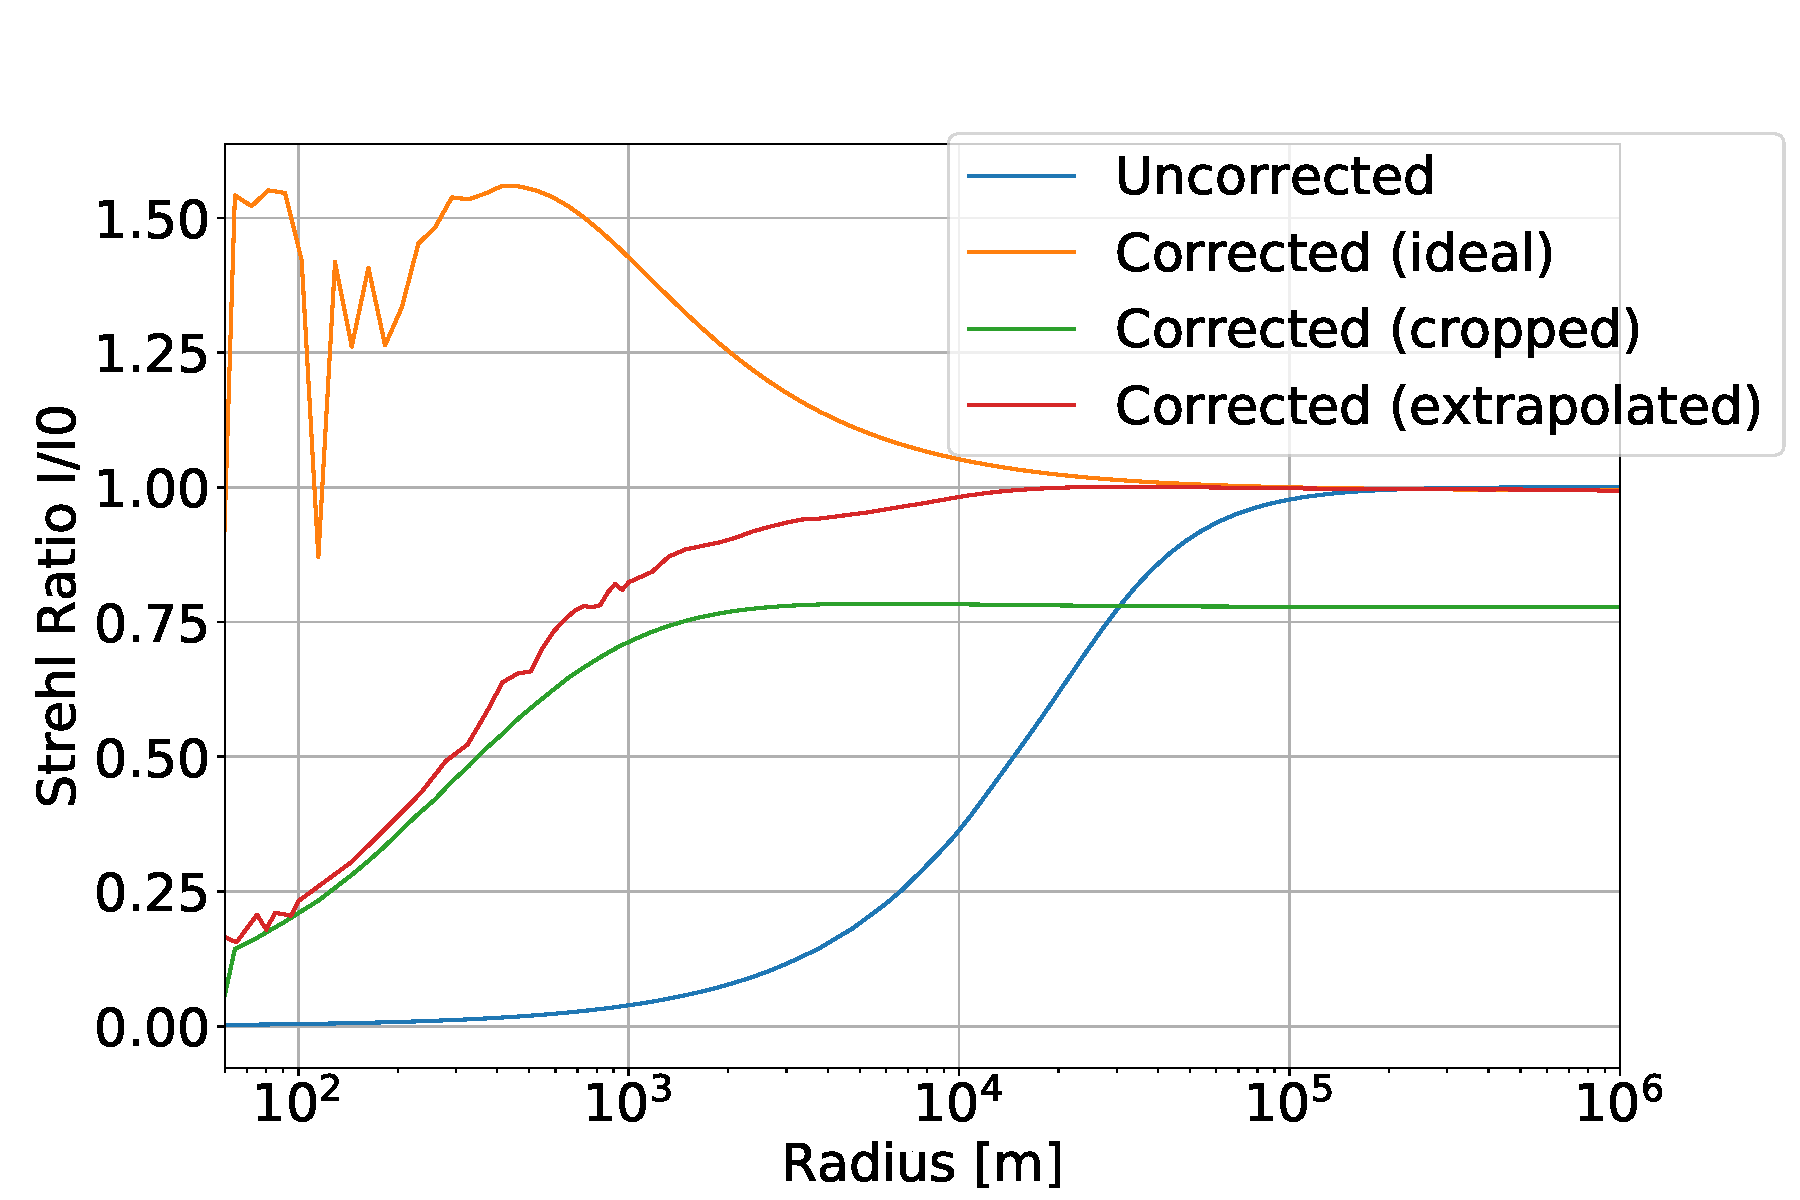
\includegraphics[width=0.99\textwidth]{figures/scan_peak_vs_negative_radius.pdf}\\
  b)\\
  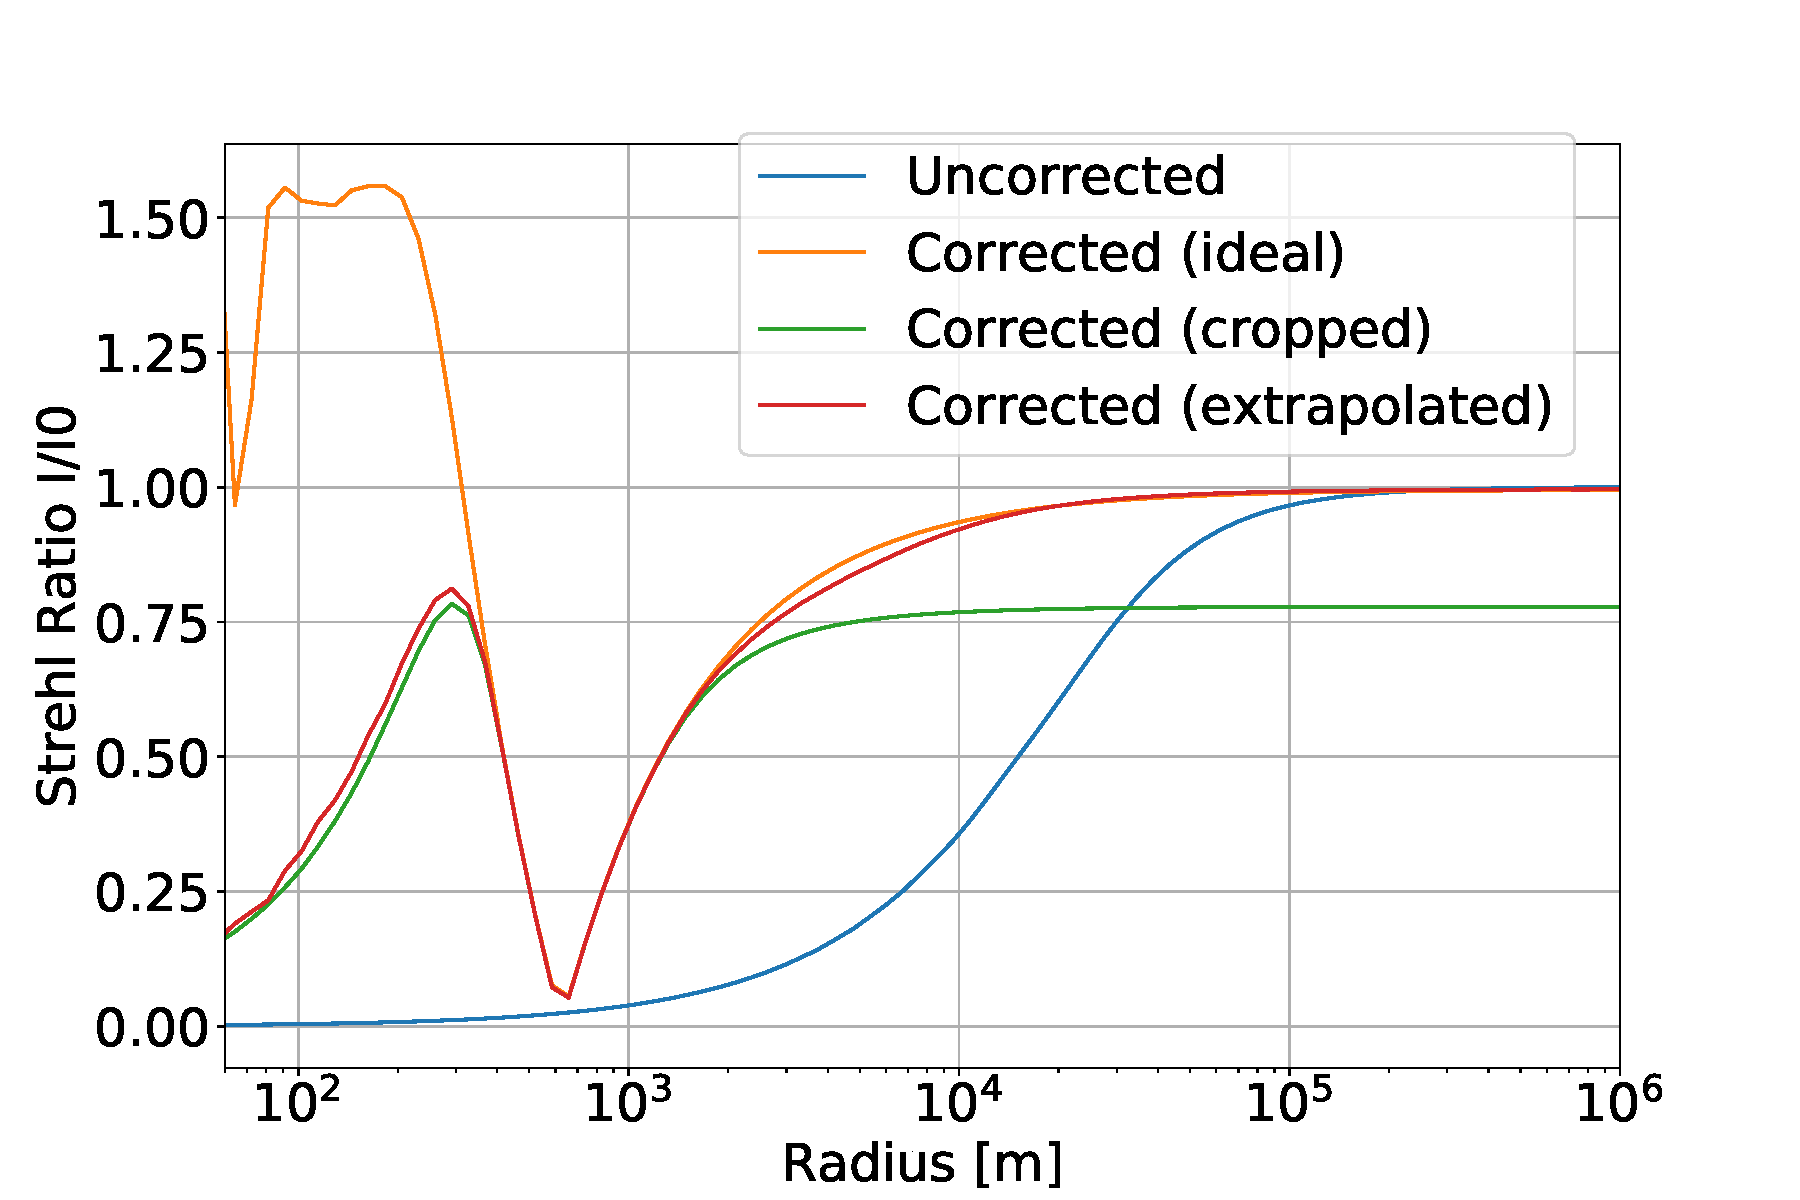
\includegraphics[width=0.99\textwidth]{figures/scan_peak_vs_positive_radius.pdf} 
  
  \end{tabular}
  \end{center}
  \caption{
Variation of the Strehl ratio at $E$=230.888~eV as a function of the deformation radius of curvature in M1 for a) convex curvature (bump) and b) concave curvature (anti-bump). Deformation is compensated with the corrective profiles in M3 expressed as a function of AXO basis for two cases: crop the profile to the AXO dimension (case A) and extrapolate the profile outside the AXO mirror (case B).}
  \end{figure} 


Next, we studied a periodic deformation in M1 with a form of cosine. The cosine is selected for having a flat top at the mirror center (a sine would give an inflection). \inblue{A }
deformation amplitude of 50 nm \inblue{is used}, independent of the period. This value has been chosen after studying a wider range of amplitudes to illustrate a case where corrections are efficient. \inblue{Deformations with small aplitudes (about 0-30 nm) give acceptable Strehl ratio (above 0.8).} We present in Fig.~\ref{fig:strehlRatioCosine} the results as a function of the number of ripples found in the mirror length. The period of the cosine is the mirror length over the number of ripples; zero ripples corresponds to the undeformed profile, which defines the normalization of Strehl ratio to one. The results may be very different if the photon energy is increased, as the geometry (illumination) changes, the diffraction effect is wavelength-dependent and also higher energies imply less coherence thus a  full coherence calculation as done here is insufficient.

For the uncorrected profiles, the intensity distribution at the focal plane will feature satellite peaks because the periodic deformation acts as a grating. These peaks are more intense for higher deformation amplitudes, thus removing more intensity in the central peak and decreasing the Strehl ratio. That makes that the curves (blue) saturate about a Strehl ratio of 0.4. The satellite peaks will separate spatially from the main peak, and the distance increases with the number of ripples (frequency), manifested in a decrease of the Strehl ratio from one (zero ripples) to a constant value at about 2--3 ripples, when the satellites completely separate from the main peak. At this point, the satellites separate more and more when increasing the number of ripples, but this does not modify the Strehl ratio, as the main peak remains constant. This is also consistent with the fact that the Strehl ratio in Marechal's approximation depends only on rms, which does not vary with the period, only with the amplitude.
%The situation changes (mentioned below) when the spatial frequency increases beyond the AXO's correction.

We study first the case of applying an ideal active correction, therefore applying the calculated profile not yet expanded on AXO basis (orange curves in Fig.~\ref{fig:strehlRatioCosine}). These corrections work efficiently in the sense that they recover satisfactory values of Strehl ratio larger than 0.8 independently of the number of ripples. One characteristic is the oscillatory behaviour of the Strehl ratio. This is originated during the migration of a satellite peak that is very narrow in width: there are positions where it is harder for the AXO to suppress or reduce it with a consequent reduction of the Strehl ratio. A second feature is that there are cases where the M1 deformation spreads the light at M3, allowing the adaptive correction to achieve an effectively higher NA, leading to an apparent Strehl Ratio above one as mentioned before.

By looking at the corrections produced by the profiles expressed as a function of the AXO orthonormal bases (Fig.~\ref{fig:strehlRatioCosine} (green and red curves), we can appreciate that the Strehl ratio drops at about 7 ripples. It is because the inability of the limited number of actuators to follow the high frequency distortion. The correction does not work for more ripples. As discussed before for the curvature, the cropped profile reduces both the integrated intensity and also the NA, making a shorter and wider peak thus decreasing the Strehl ratio to unacceptable values below 0.8.
Another feature is that the correction using a extrapolated profile looks very noisy. This is explained by the slope of the extrapolated part (the mirror edges) that is determined by the slope of the edge points, which change drastically versus the number of ripples, thus giving rise to fluctuations in the peak intensity and consequently in the Strehl ratio.
%I came across something in line 484 that is worth discussing. The optimization we perform is a minimization that reduces the rms WFE. We do this because the SR is proportional to (1 - rms). So minimizing rms maximizes Strehl. However, this works only for small rms values. It may be that when the rms is large, or the correction cannot correct well enough, or the amplitude is spread around in a peculiar way, then the correction violates our assumptions. It’s important therefore to talk about the role of the amplitude weighting in the fit.


\inblue{These results demonstrate that the correction works in a limited range of spatial frequencies (up to 5-7 ripples), but this range depends on the mirror conditions such as photon energy and deformation amplitude. 
In principle, higher spatial frequency correction could be accomplished with a longer mirror containing a greater number of electrodes.}
 
  \begin{figure}
  \label{fig:strehlRatioCosine} 
  %\begin{flushleft}
  %a)~~~~~~~~~~~~~~~~~~~~~~~~~~~~~~~~~~~~~~~~~~~~~~~~~~~~~~~b)\\
  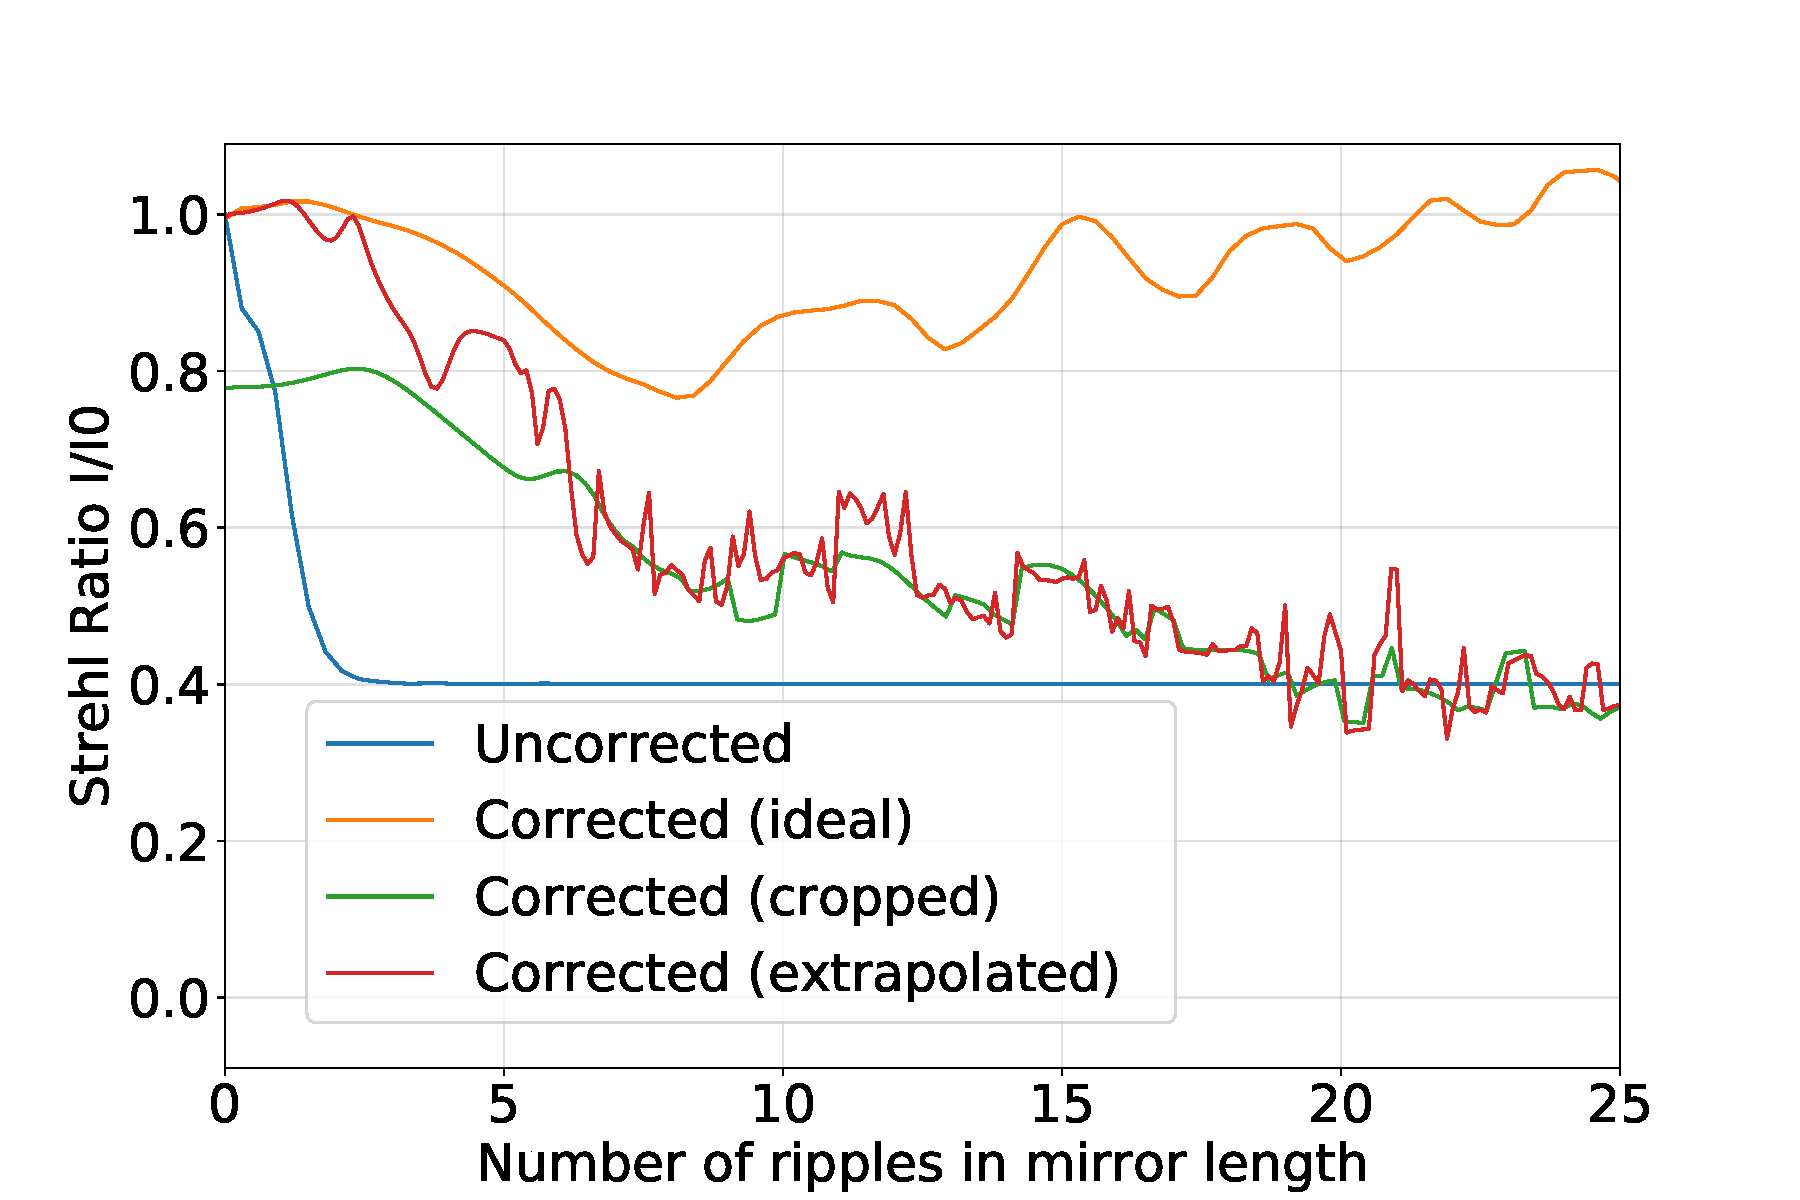
\includegraphics[width=0.99\textwidth]{figures/scan_peak_vs_cos50.pdf}
  %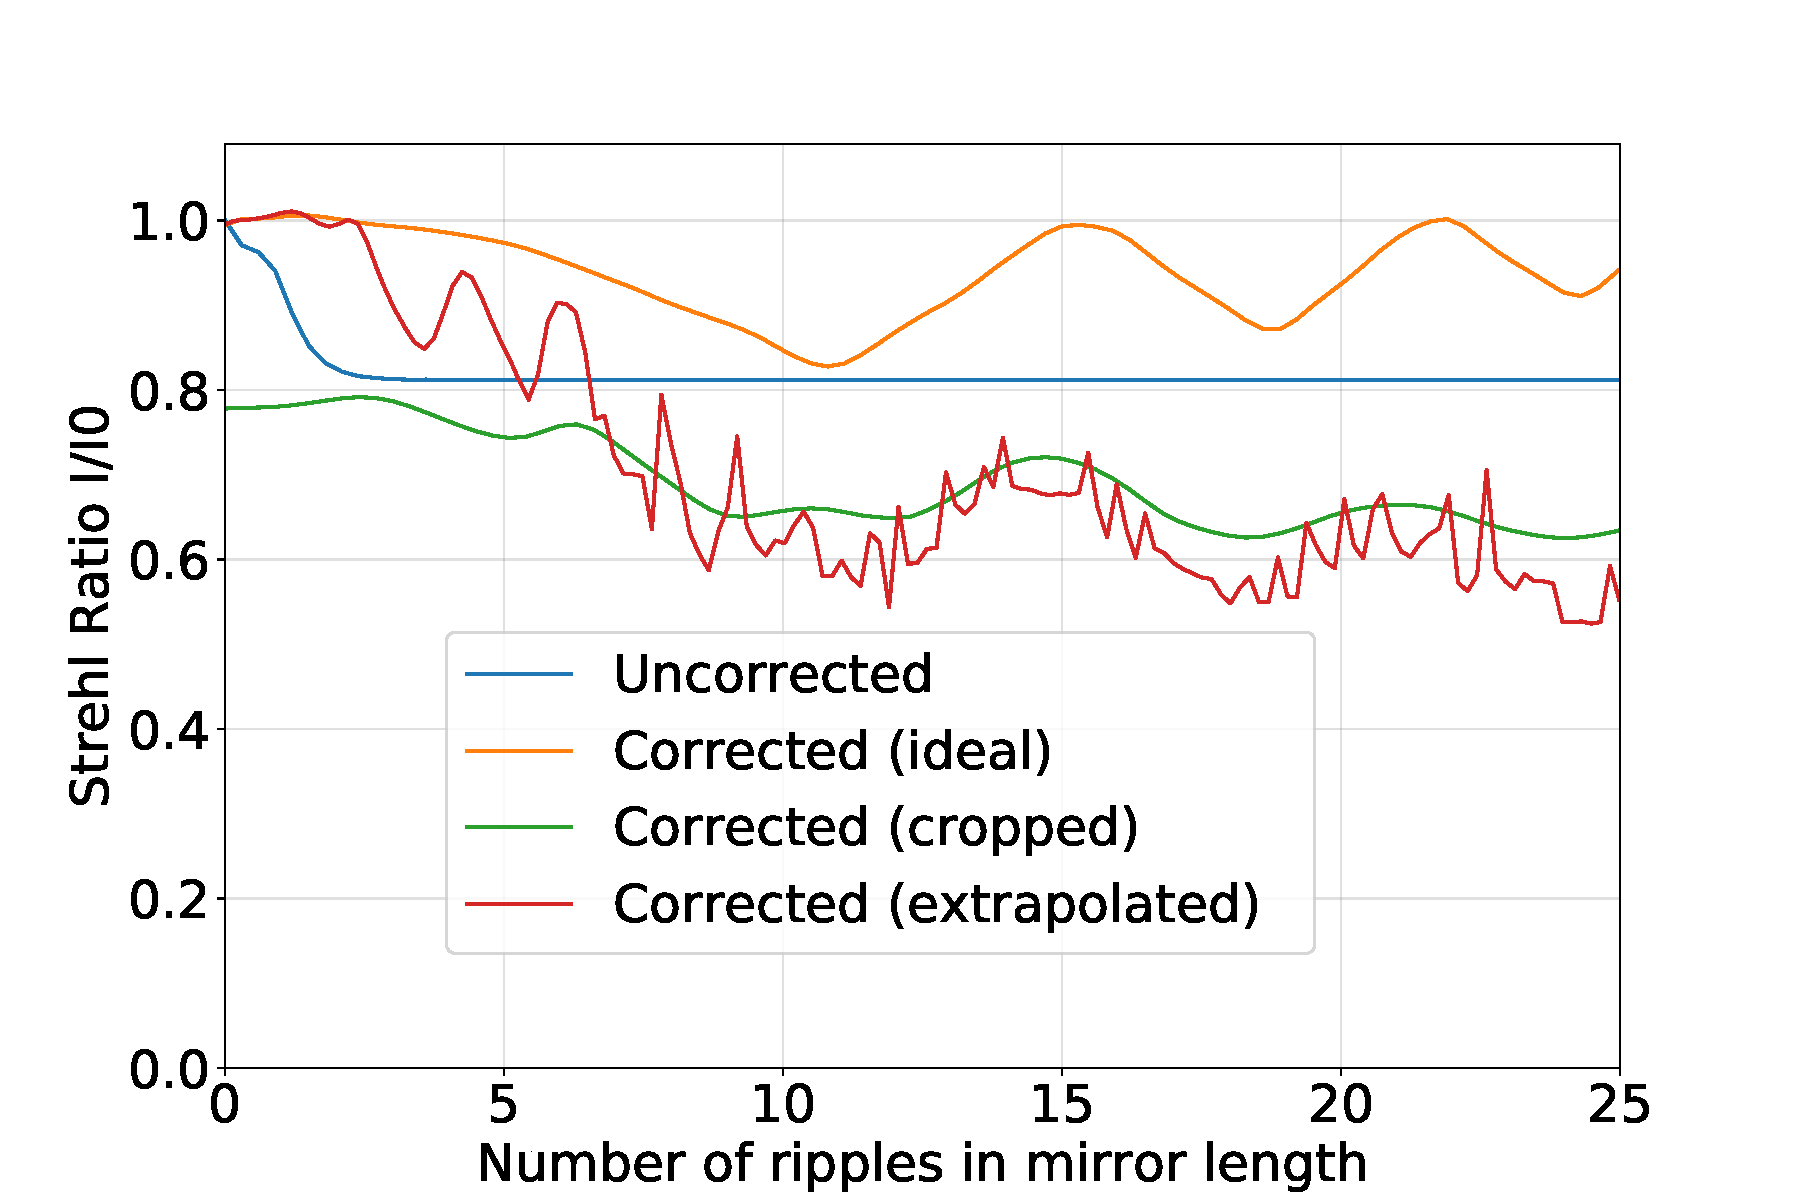
\includegraphics[width=0.49\textwidth]{figures/scan_peak_vs_cos30.pdf}
  %\end{flushleft}
  \caption{Variation of the Strehl ratio for a deformation in form of cosine with a deformation amplitude of 50 nm \inblue{corrected with different profiles at M3: ideal correction, and profiles resulting from applying the AXO basis with (cropped or extrapolated, see text).}}
  \end{figure} 

%
%
%
\section{Simulation of the full beamline}
\label{sec:2D}

For completeness, we simulate the beamline in the vertical plane, featuring a grating monochromator. It consists of a plane M2 mirror deflecting vertically, and a VLS grating that focuses the first diffracted order to the focal plane (exit slit). The role of M2 is to adjust the total deflecting angle of the monochromator (constant deflecting angle) when the VLS grating is rotated to change photon energy. For the simulations we can completely ignore it as it is not an optically active element given that i) it does not crop the beam, and ii) its surface is supposed to be perfect. The VLS grating is placed at $p$=25.73~m from the source and $q$=4.239~m from the focus. The parameters of the VLS optimized for working at E=230.888~eV are: $g_0$=300~lines/mm, $g_1=$ 0.2698~mm$^{-2}$, and $g_3$=8.7715 10${^{-5}}$~mm$^{-3}$, and the angles are $\alpha$=87.127\textdegree, $\beta$=-85.660\textdegree and $\theta=(\alpha-\beta)/2$= 86.3936\textdegree ~(c=$\cos \beta / \cos \alpha$=1.51). The grating is defined by a profile made with step functions of 10~nm height (ruled grating) over a mesh covering the grating length of 150~mm (Fig.~\ref{fig:grating}a). The effect of the grating diffraction is calculated using the model described in section~\ref{sec:grating}. The intensity distribution after the grating diffraction is in Fig.~\ref{fig:grating}b which shows a well-focused image with FWHM=4.41$\mu$m. These results are in good agreement with other simulations for the grating made with the wave optics code WISEr \cite{Raimondi2014} or the ray-tracing SHADOW.

  \begin{figure}
  \label{fig:grating} 
  \begin{flushleft}

  a)~~~~~~~~~~~~~~~~~~~~~~~~~~~~~~~~~~~~~~~~~~~~~~~~~~~~~~~~~b)
  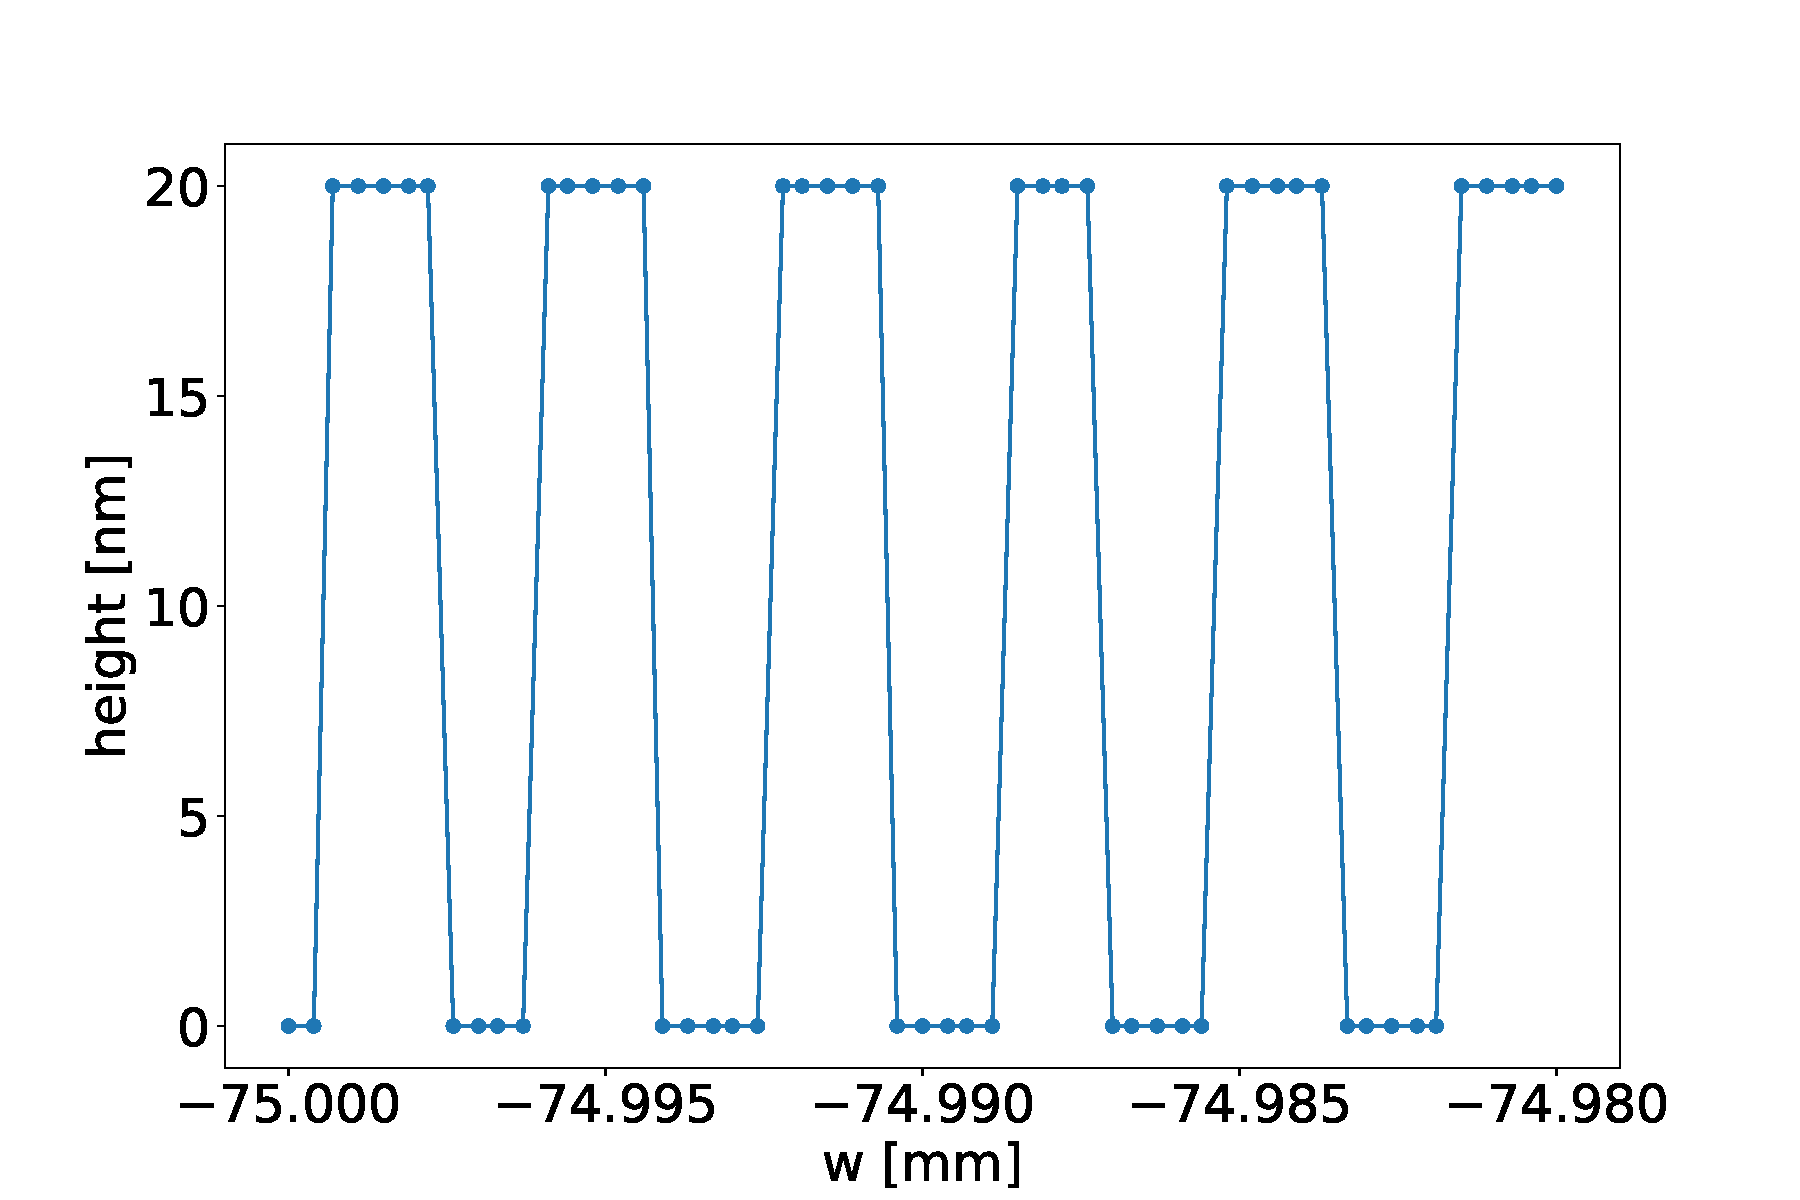
\includegraphics[width=0.48\textwidth]{figures/grating.pdf} 
   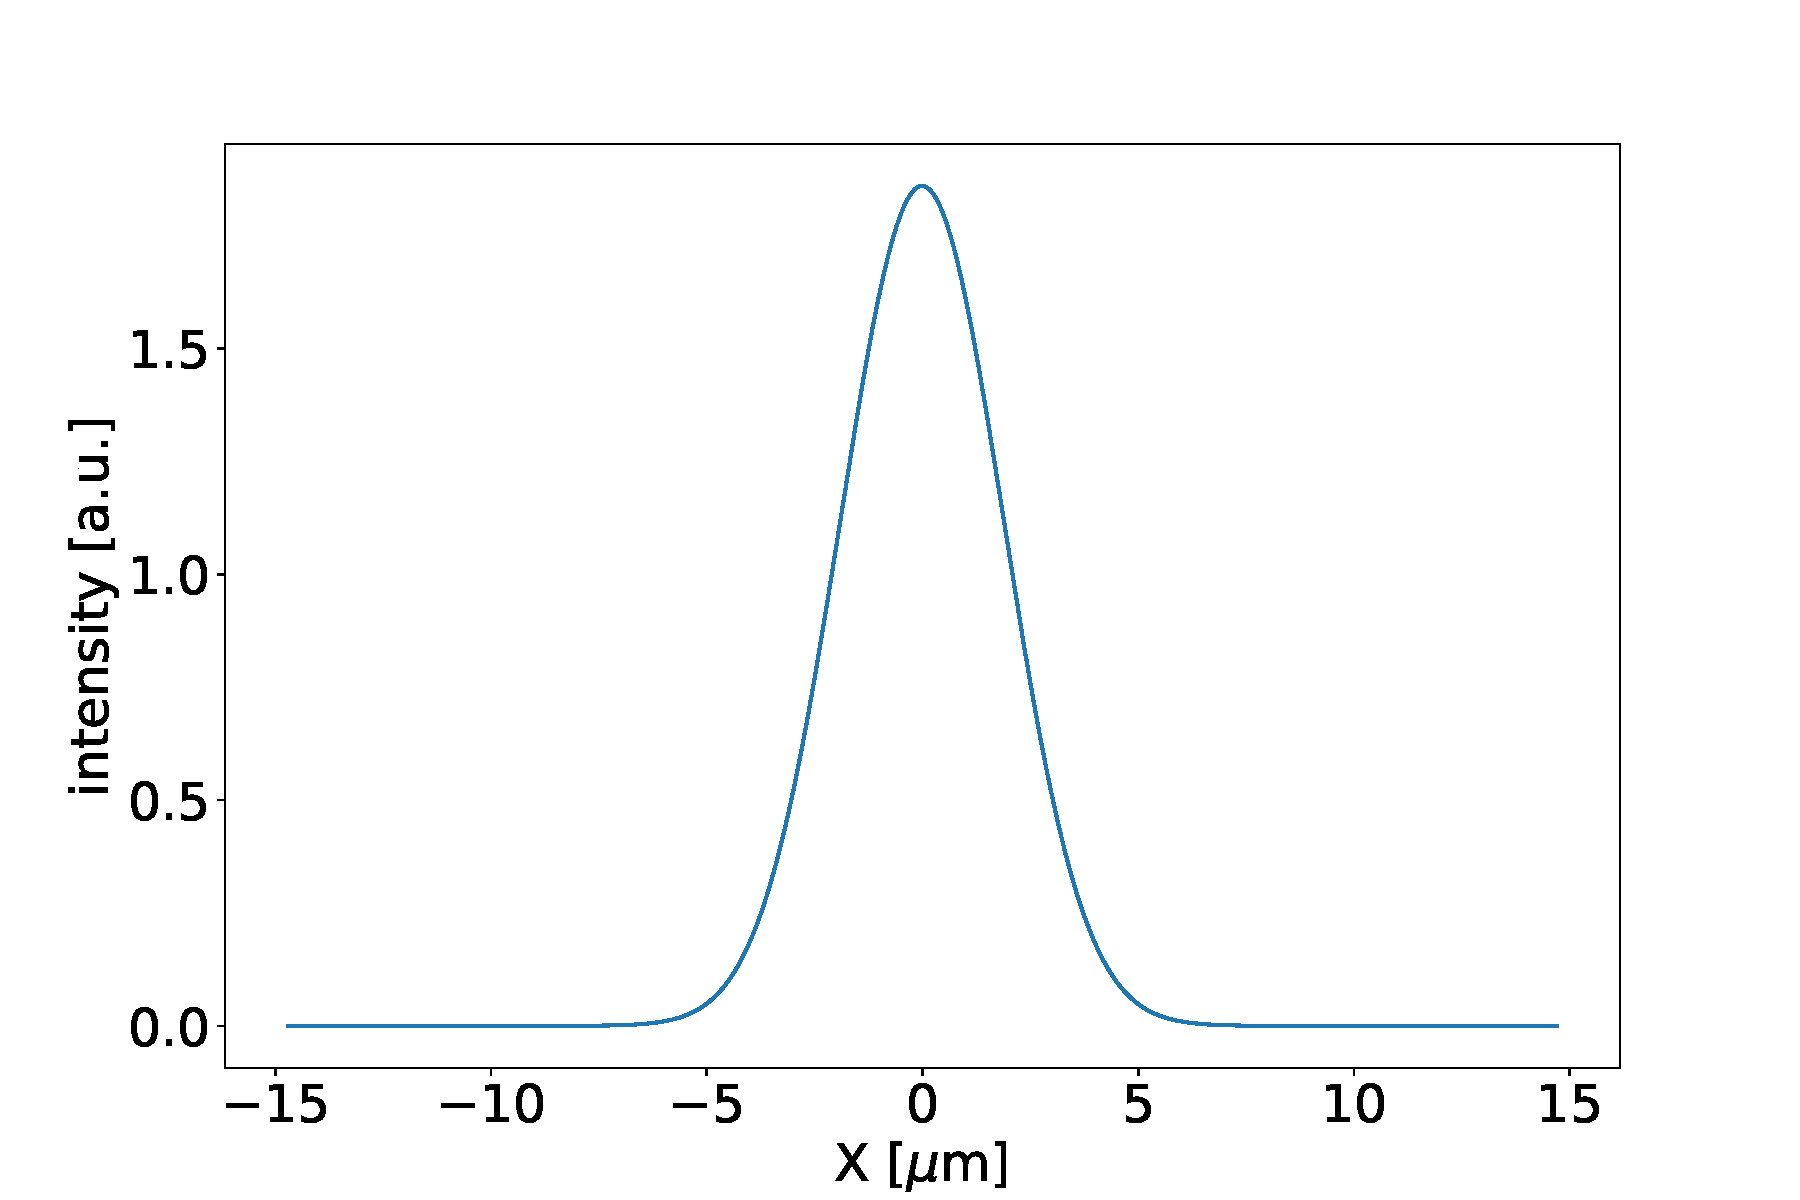
\includegraphics[width=0.48\textwidth]{figures/intensitygrating.pdf}
  \end{flushleft}
  \caption{ a) VLS profile used for the simulations (fragment). The total VLS grating length is 150 mm and contains 5 10$^5$ points. b) Intensity profile at the image position (exit slit) produced by the VLS grating.}
  \end{figure}

The simulations for the vertical plane are combined with the results for the horizontal plane (Fig.~\ref{fig:nodeformation} or \ref{fig:intensitycorrected}) for making a 2D plot. This is done via the outer product of the horizontal and vertical profiles. Fig.~\ref{fig:intensity2D} shows the results for the worst case of deformation (vertical polarization with water cooling) before and after correction. 

  \begin{figure}
  \label{fig:intensity2D} 
  \begin{flushleft}
  \begin{tabular}{l} 
  a)~~~~~~~~~~~~~~~~~~~~~~~~~~~~~~~~~~~~~~~~~~~~~~~~~~~~~~~~~~b)\\
  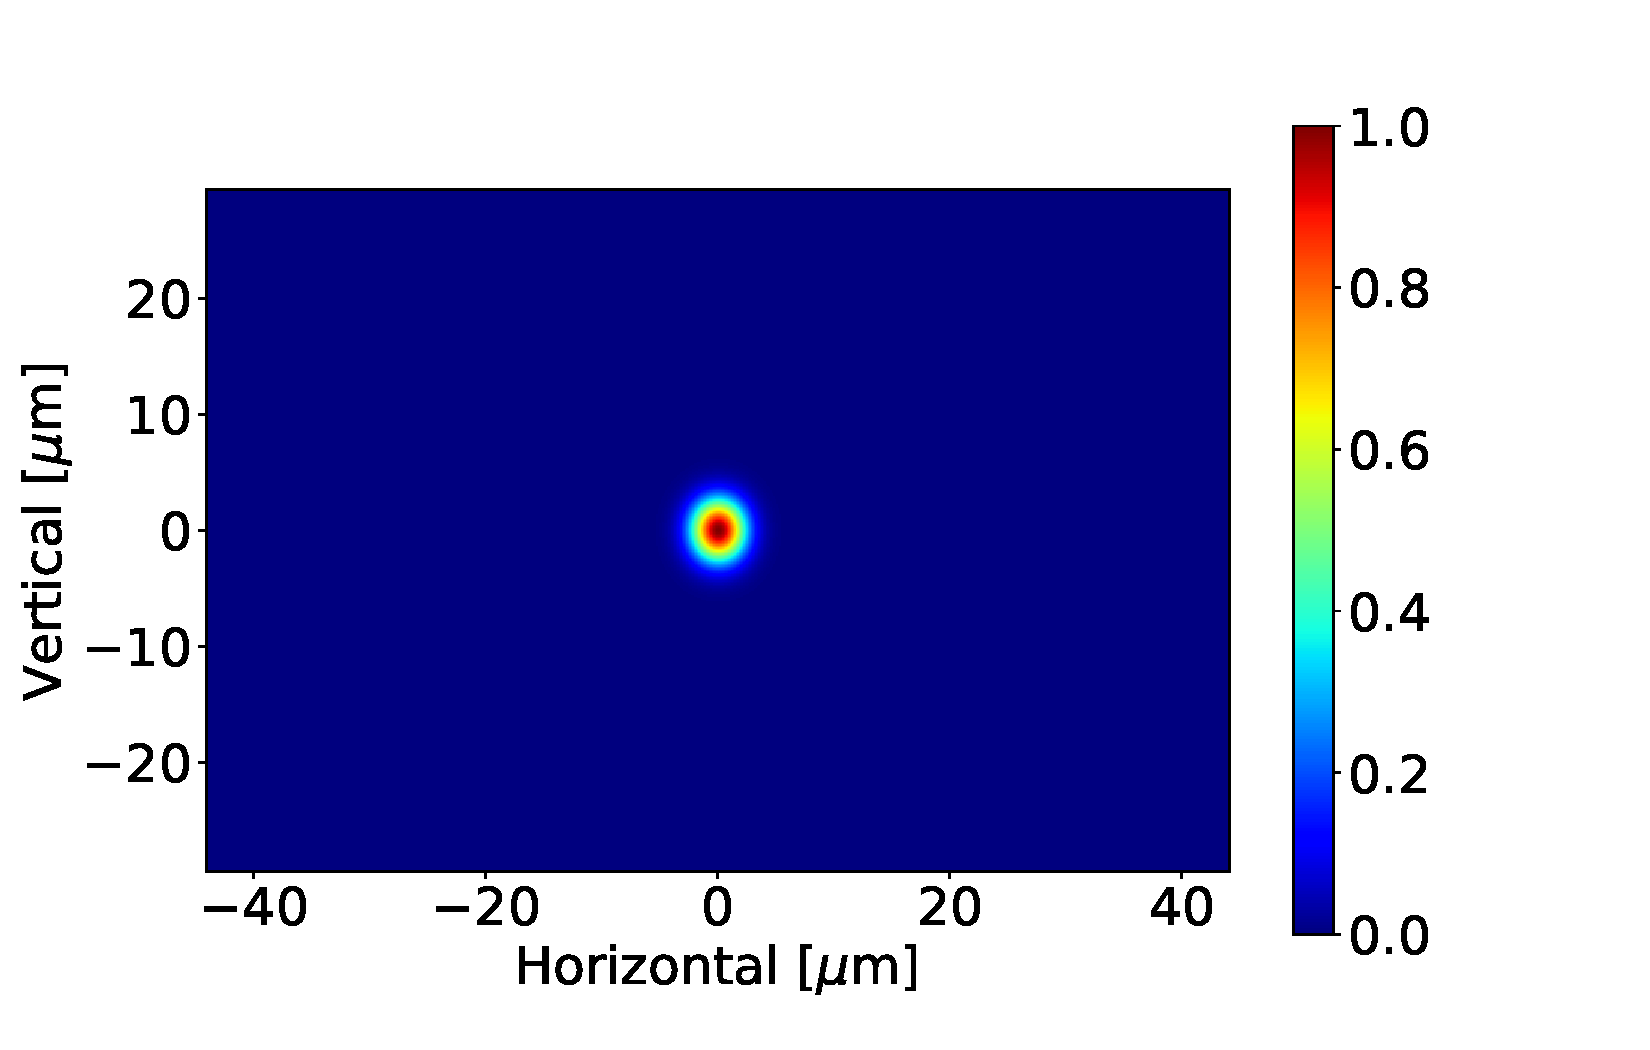
\includegraphics[width=0.5\textwidth]{figures/intensity2Duncorrected.pdf}
  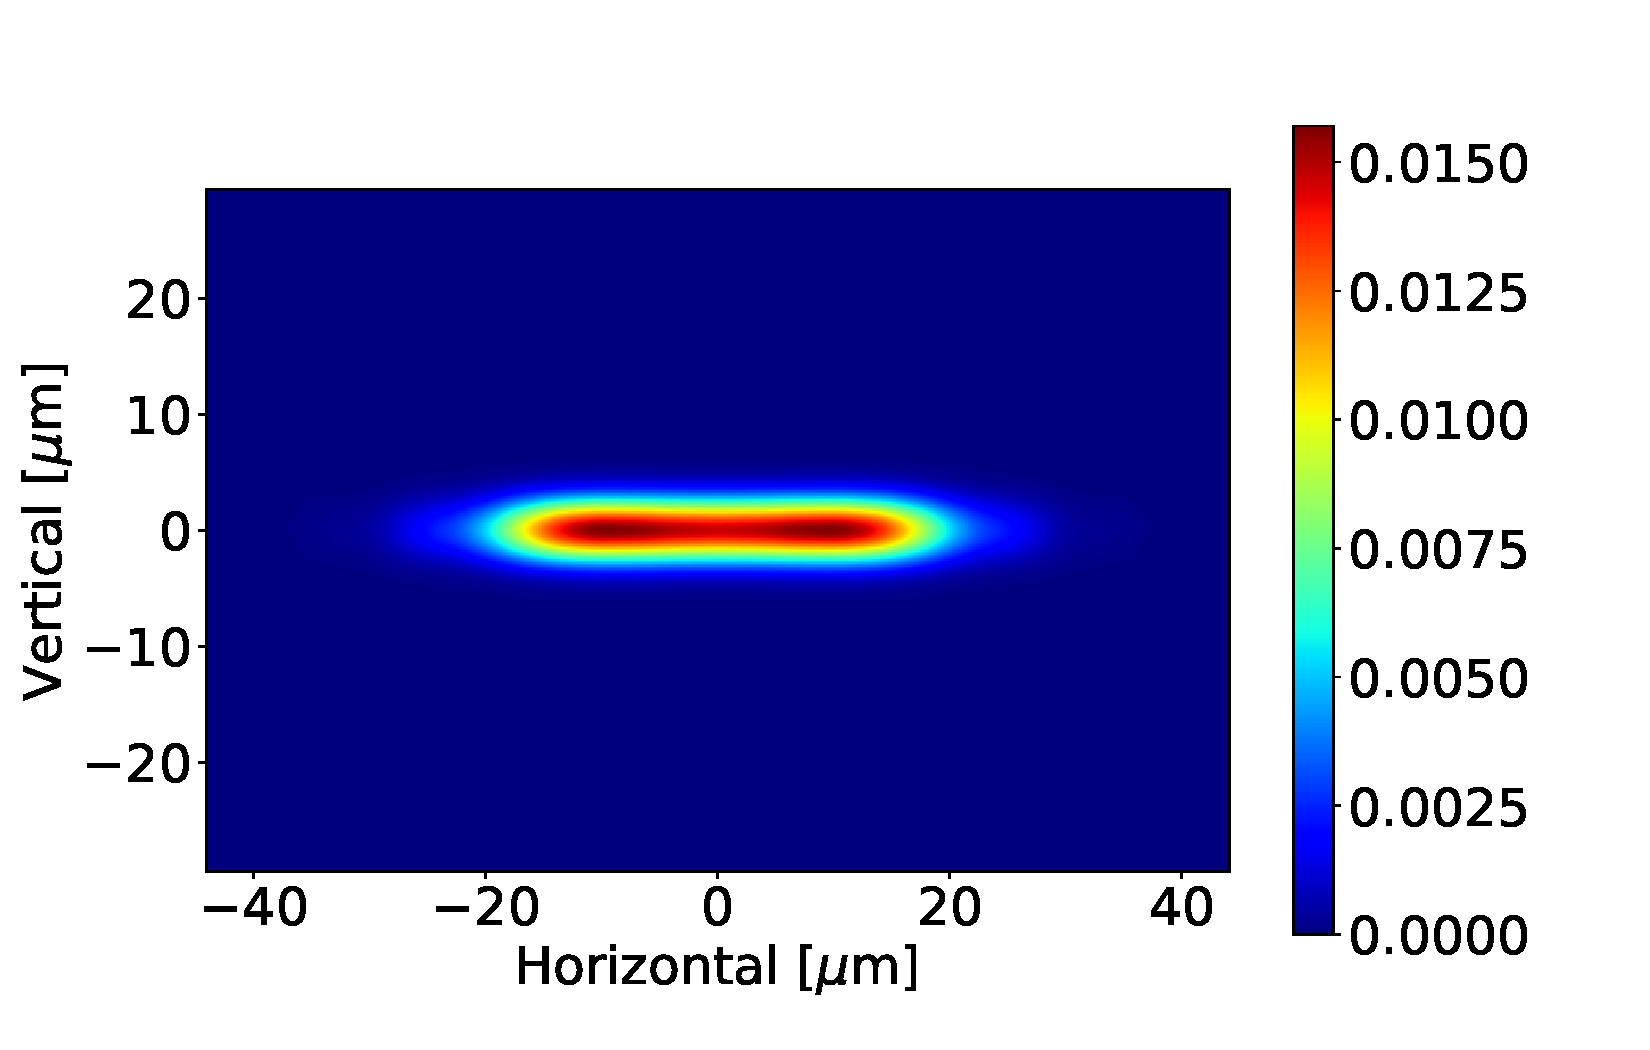
\includegraphics[width=0.5\textwidth]{figures/intensity2Dcorrected.pdf}

  \end{tabular}
  \end{flushleft}
  \caption{2D intensity at the image position (exit slit plane) obtained for the worst deformation case (vertical polarization and water cooled M1) a) uncorrected image. b) corrected image by using M3 AXO. These images have been obtained combining the vertical profile (Fig.~\ref{fig:grating})) with the uncorrected and corrected horizontal profiles (Figs.~\ref{fig:nodeformation} and \ref{fig:intensitycorrected}, respectively.) }
  \end{figure}
  
%
%
%
\section{Summary and conclusions}
\label{sec:summary}

This work demonstrates the potential efficacy of downstream adaptive optics for correcting wavefront errors introduced by upstream optical elements, across a range of error magnitudes that would be large in practice.

For this study we developed a simple model to simulate a beamline using 1D wavefront propagation. The theoretical models used are presentedin section~\ref{sec:wofry}. The code developed is fully implemented in the WOFRY package in OASYS. We analyzed the degradation of the beamline parameters, in particular intensity distribution and Strehl ratio at focus, due to the thermal load of the white beam mirror M1, and various other aberration cases. We showed that in the case of cryogenic cooling of the M1 mirror, the performance remains close to the ideal (undeformed) case, therefore no downstream wavefront correction is needed. However, if the M1 mirror is water-cooled, the induced heat load errors significantly disturb the intensity distribution at the focal plane.

Our analysis, conducted with 230.888 eV photon energy, shows that wavefront disturbances can be corrected using adaptive X-ray optics, as verified by simulating a realistic model of wavefront correction by an adaptive X-ray mirror. Furthermore, we analyzed the M1 deformation range over which the adaptive optics work, by scanning the M1 deformations modelled as curvature (bump or anti-bump) and waviness. We showed that curvatures can be effectively corrected for radii greater than 100~m. The simulations done with wavy profiles show than low spatial frequencies can be corrected, in an optimal mode up to 2--3 ripples per mirror length, and in a satisfactory way (providing Strehl ratio greater than 0.8) up to 5--7 ripples per mirror length. However, the geometry of the adaptive mirror featuring 18 actuators covering a length of 140~mm cannot correct spatial frequencies above 7 ripples across the mirror length. The proposed model helped to demonstrate the suitability and limitations of using an adaptive mirror to correct for wavefront deformations originated upstream of it. This approach can be broadly applied to beamlines with adaptive elements. We recommend such studies be conducted to establish the correctable range of errors as a function of photon energy, across a beamline's operating energy range.

\inblue{OASYS workspaces and scripts used for calculations and graphics in this work are available in the repository {\tt https://github.com/oasys-als-kit/Paper\_JSR\_yi5097}.}
%However, because our water-cooled finite element model does not include a mounting or cooling system, the presented results should be seen as a `best' or idealized case.  In other words, the shape of an actual water-cooled mirror will be more difficult to correct than what the calculations in this model indicate. In contrast, our model of the liquid-nitrogen-cooled mirror does includes mounting and cooling system deformation, and therefore is a more realistic model than what is presented for the water-side-cooled case.

%\acknowledgments % equivalent to
\section{Ackowledgements}       
 
 
This work was supported by the Director, Office of Science, Office of Basic Energy Sciences, of the U.S. Department of Energy under Contract No. DE-AC02-05CH11231.
 
% References
\bibliographystyle{iucr} % makes bibtex use spiebib.bst
\bibliography{report} % bibliography data in report.bib

\end{document} 
